\documentclass[11pt,a4paper]{article}

% Packages
\usepackage[utf8]{inputenc}
\usepackage[T1]{fontenc}
\usepackage{amsmath, amssymb, amsfonts}
\usepackage{geometry}
\geometry{a4paper, margin=2.5cm}
\usepackage{xcolor}
\usepackage{tcolorbox}
\tcbuselibrary{skins, breakable, theorems} 
\usepackage{hyperref}
\usepackage{graphicx}
\usepackage{enumitem}
\usepackage{tabularx}
\usepackage{float}
\graphicspath{{./Images/}}

% Colors setup
\definecolor{sapienzared}{RGB}{130, 36, 51}
\definecolor{theoryblue}{RGB}{20, 60, 120}
\definecolor{practicegreen}{RGB}{30, 100, 50}
\definecolor{highlightorange}{RGB}{230, 120, 20}

% Custom Box Environments
\newtcolorbox{theorybox}[1]{
    colback=theoryblue!5,
    colframe=theoryblue,
    fonttitle=\bfseries,
    title=#1,
    arc=3mm,
    breakable
}

\newtcolorbox{recipebox}[1]{
    colback=practicegreen!5,
    colframe=practicegreen,
    fonttitle=\bfseries,
    title=#1,
    arc=3mm,
    breakable
}

\newtcolorbox{examtip}{
    colback=sapienzared!5,
    colframe=sapienzared,
    fonttitle=\bfseries,
    title=Exam Tip / Oral Question Alert!,
    arc=1mm,
    leftrule=3mm
}

% Title
\title{\textbf{\Huge Robotics 2}}
\author{Based on Prof. De Luca's Lectures}
\date{\today}

\begin{document}

\maketitle
\tableofcontents
\newpage

% ==========================================
% PART 1: THEORY
% ==========================================
\part*{Theory Core Concepts}

% ---------------------------------------------------------
\section{Kinematic Calibration}
\textbf{The Goal:} Calibration aims to improve the \textbf{absolute accuracy} of a robot via software by correcting the nominal Denavit-Hartenberg (DH) parameters. Note that calibration \textit{cannot} improve \textbf{repeatability}, which depends entirely on the mechanical quality of the hardware (e.g., backlash, component stiffness).

\textbf{Sources of Error:} Discrepancies between the real and computed end-effector pose arise from manufacturing tolerances, assembly errors, and factory encoder offsets (which shift the "zero" reference). In an open kinematic chain, these errors amplify as we move towards the end-effector.

\textbf{The Math \& Dimensions:} Since direct kinematics is highly non-linear, we linearize it using a first-order Taylor expansion. The resulting basic calibration equation for a single measurement is:
\begin{equation}
    \Delta y_e = \Phi(q) \Delta \xi
\end{equation}
\begin{itemize}
    \item $\Delta y_e$: The measured Cartesian error. It is a $6 \times 1$ vector (3 position coordinates + 3 orientation coordinates).
    \item $\Delta \xi$: The vector of unknown parameter errors. For a robot with $n$ joints, there are 4 DH parameters per joint ($\alpha, a, d, \theta$). Thus, $\Delta \xi$ is a $4n \times 1$ vector.
    \item $\Phi(q)$: The \textbf{Regressor Matrix}. Since it maps a $4n$ vector to a $6$ vector, its dimensions are exactly $\mathbf{6 \times 4n}$. It is built using the partial derivatives of the direct kinematics evaluated at the nominal parameters.
\end{itemize}

\textbf{The Stacking Procedure (The "Bar" Variables):} A single measurement yields at most 6 equations, which is utterly insufficient to find $4n$ unknowns. Therefore, we measure the robot in $l$ different configurations (with $l \gg n$). We "stack" all these measurements into a massive block equation, denoted by the bar notation:
\begin{equation}
    \overline{\Delta y_e} = \overline{\Phi} \Delta \xi
\end{equation}
Now $\overline{\Delta y_e}$ is $6l \times 1$ and $\overline{\Phi}$ is $6l \times 4n$. We have transformed the problem into a heavily overdetermined linear system, which we solve using the pseudoinverse (Least Squares) to find the parameter errors: $\Delta \xi = \overline{\Phi}^\# \overline{\Delta y_e}$. This guarantees the minimum norm of the residual estimation error.

% ---------------------------------------------------------
\section{Kinematic Redundancy}
\textbf{Redundancy is Relative:} A robot is never redundant "in absolute terms". It is redundant \textit{with respect to a specific task}. If the number of joints $n$ is strictly greater than the dimension of the task $m$ ($n > m$), the robot is redundant. Consequently, the differential kinematics $\dot{x} = J(q)\dot{q}$ admits infinite solutions.

To resolve redundancy at the velocity level, we rely on one fundamental equation that dictates the entire theory:
\begin{equation}
    \dot{q} = J^\# \dot{x} + (I - J^\# J)\dot{q}_0
\end{equation}
This formula is composed of two fundamental blocks:
\begin{enumerate}
    \item \textbf{The Minimum Norm Term ($J^\# \dot{x}$):} Using the Moore-Penrose pseudoinverse $J^\# = J^T(JJ^T)^{-1}$, this provides the exact joint velocities strictly necessary to execute the primary task. 
    \textit{What does "Minimum Norm" mean?} It does NOT mean minimum task error. It means that among all infinite ways to move the motors to achieve $\dot{x}$, this solution minimizes the scalar value $\|\dot{q}\|^2 = \dot{q}_1^2 + \dots + \dot{q}_n^2$. It is the most "lazy" and efficient solution.
    
    \item \textbf{The Null-Space Playground ($(I - J^\# J)\dot{q}_0$):} The matrix $(I - J^\# J)$ is an orthogonal projector. It takes \textit{any} arbitrary velocity vector $\dot{q}_0$ and mathematically "erases" the parts that would disturb the primary task. What remains is a \textbf{self-motion} (internal reconfiguration) that leaves the end-effector perfectly still.
\end{enumerate}

\subsection{The Weighted Pseudoinverse}
The standard pseudoinverse treats all joints equally. The Weighted Pseudoinverse introduces a diagonal matrix $W > 0$, minimizing the weighted sum $\dot{q}^T W \dot{q}$. It is used in 4 specific scenarios:
\begin{enumerate}
    \item \textbf{Mixing Units:} When a robot has both prismatic (m/s) and revolute (rad/s) joints, summing them in a standard norm makes no physical sense. $W$ normalizes the units.
    \item \textbf{Penalizing Heavy/Slow Joints:} By assigning a high weight to a massive base joint and a low weight to a light wrist, the algorithm will prefer moving the wrist, saving huge amounts of energy.
    \item \textbf{Joint Limit Avoidance:} By making weights dynamically approach infinity as a joint nears its mechanical limit, the algorithm "understands" that moving that joint has become too costly and halts it smoothly.
    \item \textbf{Minimizing Actual Kinetic Energy:} If we set $W = M(q)$ (the Inertia Matrix), the algorithm physically minimizes the true instantaneous Kinetic Energy of the robot: $T = \frac{1}{2}\dot{q}^T M(q) \dot{q}$.
\end{enumerate}

% ---------------------------------------------------------
\subsection{Singularity Robustness: Damped Least Squares}
\textbf{The Problem:} The pseudoinverse is computed via Singular Value Decomposition (SVD). It divides by the singular values $\sigma_i$ of the Jacobian ($1/\sigma_i$). Near a singularity, $\sigma_i \to 0$, causing the required joint velocities to explode to infinity.

\textbf{The Solution:} The Damped Least Squares (DLS, or Levenberg-Marquardt) method abandons the "perfect" minimum norm solution. Instead of ensuring zero task error, it minimizes a mixed objective function: $H = \|\dot{x} - J\dot{q}\|^2 + \mu^2 \|\dot{q}\|^2$, where $\mu^2$ is a damping factor. The formula becomes:
\begin{equation}
    \dot{q}_{DLS} = J^T(J J^T + \mu^2 I)^{-1} \dot{x}
\end{equation}
The term $+\mu^2 I$ guarantees the matrix is always invertible, even in full singularity!

\textbf{Behavior of the SVD values (Crucial for Exams)}
The DLS maps the singular values using the function $\frac{\sigma_i}{\sigma_i^2 + \mu^2}$. This creates 3 behavioral zones:
\begin{itemize}
    \item \textbf{Far from singularity ($\sigma_i \gg \mu$):} The function acts like $1/\sigma_i$. DLS behaves exactly like the standard pseudoinverse. Perfect tracking.
    \item \textbf{Near singularity ($\sigma_i \approx \mu$):} Instead of going to infinity, the curve peaks at a maximum value of $\frac{1}{2\mu}$. Velocities are capped. The robot safely deviates slightly from the task to protect the hardware.
    \item \textbf{Exactly at singularity ($\sigma_i \to 0$):} The value smoothly drops to $0$. The robot halts smoothly along singular directions. Tracking error is high, but the hardware is 100\% safe.
\end{itemize}
 

% ---------------------------------------------------------
\subsection{Handling Multiple Tasks and Bounds}
When we have multiple Cartesian tasks or hard physical limits, we have four main architectures. Understanding the flaws of the first two is key to understanding why we use the last two.

\begin{enumerate}
    \item \textbf{Task Augmentation (Brute Force):} We stack Task 1 ($J_1$) and Task 2 ($J_2$) into a single augmented matrix $J_A$. We solve with $\dot{q} = J_A^\# \dot{x}_A$. 
    \textit{The Flaw:} It treats all tasks equally. If tasks conflict (not enough DOFs), the pseudoinverse yields a Least Squares compromise. The robot will fail \textit{both} tasks.
    
    \item \textbf{Extended Jacobian (The Square Way):} We stack tasks until $J_{ext}$ is exactly $n \times n$, then use the standard inverse $J_{ext}^{-1}$. It guarantees cyclic repeatability.
    \textit{The Flaw:} Fatal algorithmic singularities. If tasks conflict, the determinant goes to zero and commanded velocities mathematically explode to infinity.
    
    \item \textbf{Task Priority (The Safe Hierarchy):} We establish a strict hierarchy. Task 1 is untouchable. Task 2 is executed \textit{strictly} within the Null-Space of Task 1. If they conflict, Task 2 elegantly yields.
    
    \item \textbf{SNS - Saturation in the Null Space (Hard Bounds):} SNS applies strict hardware limits (e.g., max motor speed). If a joint exceeds its limit, SNS saturates it at $V_{max}$, removes that joint from the equation, and uses the Null-Space of the remaining joints to re-route the motion and complete the task safely.
\end{enumerate}

\subsubsection{Deep Dive: The Mathematics of Task Priority}
Let primary task be $\dot{y}_1 = J_1 \dot{q}$ and secondary be $\dot{y}_2 = J_2 \dot{q}$. The rigorous Maciejewski-Siciliano formulation is:
\begin{equation}
    \dot{q} = J_1^\# \dot{y}_1 + (I - J_1^\# J_1) \left[ J_2(I - J_1^\# J_1) \right]^\# (\dot{y}_2 - J_2 J_1^\# \dot{y}_1)
\end{equation}
Let's break down this complex formula:
\begin{itemize}
    \item \textbf{The Untouchable Block ($J_1^\# \dot{y}_1$):} The minimum norm velocity to execute Task 1 perfectly.
    \item \textbf{The Residual Error ($\dot{y}_2 - J_2 J_1^\# \dot{y}_1$):} While the robot executes Task 1, its arms move. This inevitable motion produces a "free" velocity at the Task 2 level, equal to $J_2 (J_1^\# \dot{y}_1)$. By subtracting this from the desired $\dot{y}_2$, we get the \textit{residual error}: exactly how much "work" is left to complete Task 2.
    \item \textbf{The Raw Solution ($\left[ J_2 \dots \right]^\# \dots$):} We take the pseudoinverse of the "projected Jacobian" and multiply it by the residual error.
\end{itemize}

\begin{examtip}
\textbf{The Engineer's Trick (Why the outer projector?)}\\
Notice that the projector $P_1 = (I - J_1^\# J_1)$ appears both \textit{inside} the pseudoinverse bracket and \textit{outside} of it. 
Mathematically, $P_1$ is \textbf{Hermitian} (symmetric) and \textbf{Idempotent} ($P_1^2 = P_1$). Because of this, the math says that $(J_2 P_1)^\# = P_1 (J_2 P_1)^\#$. Therefore, the outer projector is theoretically redundant! 

\textbf{So why write it?} \textit{Numerical Robustness}. Computing a pseudoinverse is heavy and generates tiny floating-point approximations in the CPU. If we omit the outer projector, these tiny math errors could "leak" out of the null-space and disturb Task 1. By applying the outer $P_1$ explicitly at the very end, we act as a final "hardware filter", wiping out any computational garbage and ensuring Task 1 remains mathematically immaculate.
\end{examtip}

\subsubsection{Generalization: Recursive Task Priority}
If we have a strict priority hierarchy of $s$ tasks ($1 < 2 < \dots < s$), writing a single massive formula becomes computationally heavy and unreadable. Instead, we use a \textbf{recursive formulation} that updates the solution step-by-step.
Let $\dot{y}_k = J_k \dot{q}$ be the $k$-th task. At step $k$, the optimal velocity that respects all previous $k-1$ higher-priority tasks is:
\begin{equation}
    \dot{q}_k = \dot{q}_{k-1} + (J_k P_{A,k-1})^\# (\dot{y}_k - J_k \dot{q}_{k-1})
\end{equation}
Where $P_{A,k-1}$ is the projector into the null-space of the \textit{augmented} Jacobian of all previous tasks. The projector itself is updated recursively:
\begin{equation}
    P_{A,k} = P_{A,k-1} - (J_k P_{A,k-1})^\# J_k P_{A,k-1}
\end{equation}
starting from $\dot{q}_0 = 0$ and $P_{A,0} = I$. This elegant recursion guarantees that the $k$-th task will \textbf{not perturb} the execution of the previous $k-1$ tasks.

% ---------------------------------------------------------
\subsection{Resolution at Acceleration Level}
Working at the velocity level ($\dot{q}$) is standard, but resolving redundancy at the \textbf{acceleration level} ($\ddot{q}$) generates smoother motions and creates a bridge to incorporate the robot's dynamics.

\textbf{The Mathematical Shift:} If the task is defined as $\dot{y} = J(q)\dot{q}$, taking the time derivative yields the task acceleration:
\begin{equation}
    \ddot{y} = J(q)\ddot{q} + \dot{J}(q)\dot{q}
\end{equation}
To isolate the joint accelerations $\ddot{q}$, we rearrange the equation: $J(q)\ddot{q} = \ddot{y} - \dot{J}(q)\dot{q}$. 

For convenience, we define the \textbf{Equivalent Task Acceleration} as $\ddot{x} \triangleq \ddot{y} - \dot{J}(q)\dot{q}$. 
The equation simply becomes $J(q)\ddot{q} = \ddot{x}$. This problem is now formally identical to the velocity-level kinematics! The general solution using the null-space projector is:
\begin{equation}
    \ddot{q} = J^\#(q)\ddot{x} + (I - J^\#(q)J(q))\ddot{q}_N
\end{equation}

\textbf{Choosing $\ddot{q}_N$:} 
\begin{itemize}
    \item \textbf{Damping:} A classic choice is to set $\ddot{q}_N = -K_D \dot{q}$ (with $K_D > 0$) to damp and stabilize the internal motions of the joints, which might otherwise drift uncontrollably.
    \item \textbf{Optimization (Discrete Time):} We can choose $\ddot{q}_N$ to locally minimize a generic performance index $G(q, \dot{q})$. Since solving this as a continuous non-linear optimal control problem is extremely hard, we solve it in \textit{discrete time} by assuming the acceleration $\ddot{q}$ is constant over a sampling interval $\Delta t$.
\end{itemize}

\textbf{Null-space Acceleration by Optimization (Discrete Time)}
\textbf{Goal:} Find the optimal $\ddot{q}_k$ to decrease $G(q, \dot{q})$ at the next step $t_{k+1}$.
Given the kinematic updates over $\Delta t$:
\begin{align*}
    \dot{q}_{k+1} &= \dot{q}_k + \Delta t \ddot{q}_k \\
    q_{k+1} &= q_k + \Delta t \dot{q}_k + \frac{1}{2} \Delta t^2 \ddot{q}_k
\end{align*}
We expand $G_{k+1}$ using a first-order Taylor series around the current state $(q_k, \dot{q}_k)$:
$$G_{k+1} \approx G_k + \nabla_q G|_k (q_{k+1} - q_k) + \nabla_{\dot{q}} G|_k (\dot{q}_{k+1} - \dot{q}_k)$$
Substituting the kinematic updates and factoring out $\ddot{q}_k$, we get:
$$G_{k+1} = G_k + \nabla_q G|_k (\Delta t \dot{q}_k) + \Delta t \left( \frac{1}{2} \Delta t \nabla_q G|_k + \nabla_{\dot{q}} G|_k \right) \ddot{q}_k$$
To maximize the decrease of $G$ (Gradient Descent), we must push $\ddot{q}_k$ in the \textbf{opposite direction} of the vector multiplying it. Thus, our optimal null-space acceleration is:
\begin{equation}
    \ddot{q}_N = -\alpha_k \left( \frac{1}{2} \Delta t \nabla_q G|_k + \nabla_{\dot{q}} G|_k \right)
\end{equation}
where $\alpha_k > 0$ is the step size.
 

\begin{examtip}
Notice the physical implication of the discrete-time formula above: to influence a cost function acting on acceleration, we must consider both the gradient w.r.t velocity ($\nabla_{\dot{q}} G$) AND the gradient w.r.t position ($\nabla_q G$). However, the position gradient is scaled by $\frac{1}{2}\Delta t$. Therefore, as the sampling time $\Delta t$ gets smaller (tends to zero), the influence of the position gradient vanishes!
\end{examtip}

% ---------------------------------------------------------
\section{Kinematic Control (Closing the Loop)}
Up to this point, we have used $\dot{y} = J\dot{q}$ assuming open-loop execution. In reality (or in simulation exercises), using pure kinematic inversion accumulates drift errors due to discrete-time integration or initial mismatches. 
To guarantee that the task is followed perfectly over time, we must close a feedback loop on the task execution error $e = y_d - y$.

\begin{itemize}
    \item \textbf{At the Velocity Level:} Instead of commanding $\dot{y}_d$ directly, we inject a proportional error correction:
    \begin{equation}
        \dot{y}_{cmd} = \dot{y}_d + K_P (y_d - y)
    \end{equation}
    where $K_P > 0$ is a positive definite gain matrix. This commanded velocity is then fed into the pseudoinverse: $\dot{q} = J^\# \dot{y}_{cmd}$.
    
    \item \textbf{At the Acceleration Level:} We replace the feedforward acceleration $\ddot{y}_d$ with a PD-like control law to ensure asymptotic tracking:
    \begin{equation}
        \ddot{y}_{cmd} = \ddot{y}_d + K_D (\dot{y}_d - \dot{y}) + K_P (y_d - y)
    \end{equation}
    This commanded acceleration is then used in the acceleration-level redundancy resolution: $\ddot{q} = J^\# (\ddot{y}_{cmd} - \dot{J}\dot{q})$.
\end{itemize}

% ---------------------------------------------------------
\subsection{Nonholonomic Mobile Manipulators (NMM)}
An NMM is a robotic arm mounted on a mobile base (usually wheeled). Solving kinematics for an NMM acts as a bridge between fixed-base robotics and mobile robotics. The key is to separate the system into two sub-components and then fuse them into a single Jacobian framework.

\subsubsection{Separation of Coordinates and Commands}
\begin{itemize}
    \item \textbf{The Mobile Base:} Described by coordinates $q_0$ (e.g., $x,y,\theta$). Because it has nonholonomic constraints (a car cannot move sideways), its kinematics are governed by a matrix $G$: $\dot{q}_0 = G(q_0)u_0$, where $u_0$ are the available base commands (e.g., linear and angular velocities).
    \item \textbf{The Manipulator Arm:} Described by joint angles $q_1$. The commands are the joint velocities themselves: $u_1 = \dot{q}_1$.
\end{itemize}
The total state vector is $q = [q_0^T \quad q_1^T]^T$, and the total available command vector is $u = [u_0^T \quad u_1^T]^T$.

\textbf{The NMM Jacobian ($J_{NMM}$)}
The end-effector velocity $\dot{y}$ depends on both the motion of the base and the motion of the arm:
$$ \dot{y} = J_0(q)\dot{q}_0 + J_1(q)\dot{q}_1 $$
By substituting the kinematic model of the base ($\dot{q}_0 = G(q_0)u_0$) and the arm ($u_1 = \dot{q}_1$), we obtain:
$$ \dot{y} = J_0(q)G(q_0)u_0 + J_1(q)u_1 $$
Factoring out the command vector $u$, we define the \textbf{NMM Jacobian}:
\begin{equation}
    \dot{y} = \underbrace{\begin{bmatrix} J_0(q)G(q_0) & J_1(q) \end{bmatrix}}_{J_{NMM}(q)} \begin{bmatrix} u_0 \\ u_1 \end{bmatrix} = J_{NMM}(q) u
\end{equation}
 

\begin{examtip}
\textbf{The NMM Golden Rule:} Once you have formulated $J_{NMM}$, the problem mathematically reverts to that of a standard fixed-base robot! 
The system is redundant if the total number of commands (dimension of $u$) is greater than the task dimension $m$. You can apply \textit{all} previously learned redundancy resolution techniques (Pseudoinverse, Null-Space, Task Priority, SNS) simply by replacing $J$ with $J_{NMM}$ and $\dot{q}$ with $u$.
\end{examtip}

% ---------------------------------------------------------
\subsection{Quadratic Programming (QP) \& Inequality Tasks}
While pseudoinverse-based methods handle linear equality constraints beautifully, they cannot natively handle strict hardware limits or bounded zones. \textbf{Quadratic Programming (QP)} is the mathematical optimization framework used to handle redundancy when both strict tasks and strict physical limits coexist.

\textbf{The Concept:} The goal of QP in robotics is to minimize a quadratic cost function (usually the kinetic energy or the joint velocity norm $\frac{1}{2}\|\dot{q}\|^2$) subject to two types of constraints:
\begin{enumerate}
    \item \textbf{Equality Constraints ($J\dot{q} = \dot{y}$):} These represent exact operational tasks. Geometrically, in the space of velocity commands, an equality constraint defines a restricted affine space (a line or a hyperplane).
    \item \textbf{Inequality Constraints ($A\dot{q} \le b$):} These represent hardware limits (e.g., $|\dot{q}| \le V_{max}$) or obstacle avoidance thresholds. Geometrically, these define a \textbf{convex area} of admissible commands.
\end{enumerate}

\subsubsection{Conflicts, Geometry, and Priorities}
\begin{itemize}
    \item \textbf{No Conflict:} If the hyperplane of the equality constraint intersects the convex area of the inequalities, an exact solution exists. The QP solver simply picks the point on that intersection closest to the origin (minimum norm).
    \item \textbf{Conflict (No Exact Solution):} If the equality hyperplane lies completely outside the convex inequality area, the task is physically impossible to execute without breaking a limit. 
\end{itemize}

When a conflict occurs, \textbf{Priority} dictates the robot's behavior:
\begin{itemize}
    \item If the \textit{inequality} has maximum priority (e.g., a hardware motor limit), the solution will stick to the boundary of the convex area. The robot will abandon perfect task execution (it slows down or deviates) to avoid breaking itself.
    \item If the \textit{equality} has maximum priority, the robot will execute the task but violate the safety limits (a theoretical condition, rarely implemented on real hardware).
\end{itemize}

\begin{figure}[H]
    \centering
    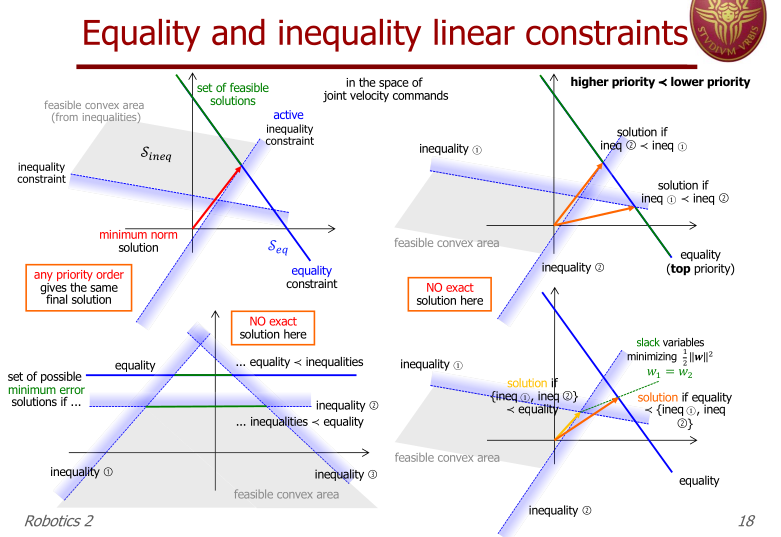
\includegraphics[width=0.8\textwidth]{QP.png}
\end{figure}

\begin{examtip}
\textbf{Slack Variables ($w$):} How does a QP solver mathematically allow a lower-priority task to fail gracefully? It uses \textbf{slack variables}. The algorithm rewrites a strict equality $J\dot{q} = \dot{y}$ as $J\dot{q} - w \le \dot{y}$. The slack $w$ absorbs the error, and the solver attempts to minimize $w$ inside its cost function to deviate from the task as little as possible.

\textbf{Hierarchical QP (HQP) and Humanoids:} Humanoid robots (like HRP-2) are the ultimate use-case for HQP. They must juggle dozens of tasks with strict life-or-death priorities: 1) Do not fall (maintain Center of Mass inside support polygon - strict inequality), 2) Avoid obstacles (strict inequality), 3) Reach for an object (equality task, lower priority). 
\end{examtip}

% ---------------------------------------------------------
\subsection{Hard Limits \& Saturation in the Null Space (SNS)}
While Quadratic Programming (QP) is the mathematically optimal framework to handle inequality constraints, solving a full Hierarchical QP at every control cycle requires massive computational power. The \textbf{SNS (Saturation in the Null Space)} method is a computationally efficient algorithmic workaround that mimics the safety of QP for box inequalities (like max joint speeds) but operates using the much faster null-space projections.

\textbf{The Concept:} The standard pseudoinverse ignores hardware bounds. If a calculated joint velocity exceeds its physical limit, we cannot simply "chop" it off. Doing so changes the direction of the velocity vector, causing the end-effector to derail from its Cartesian path.

\textbf{The Mathematical Formulation of SNS}
To mathematically "turn off" (saturate) a joint without derailing the task, the SNS algorithm uses three key components:

\textbf{1. The Selection Matrix $W$:} A diagonal matrix used to select which joints are free and which are saturated.
\begin{itemize}
    \item $W_{jj} = 1$ if joint $j$ is "free" (below its limit).
    \item $W_{jj} = 0$ if joint $j$ violates its limit and must be saturated.
\end{itemize}
Multiplying the Jacobian by $W$ creates $JW$, which effectively ignores the columns of the saturated joints.

\textbf{2. The Command Components ($a$ and $b$):} 
When joints are saturated, their motion still affects the end-effector. The remaining free joints must \textit{compensate} for this. We split the velocity command into two parts:
\begin{itemize}
    \item \textbf{The Task Execution Vector ($a$):} $a = (JW)^\# \dot{x}$. This is the primary command required for the free joints to execute the desired task $\dot{x}$.
    \item \textbf{The Compensation Vector ($b$):} $b = (I - (JW)^\# J)\dot{q}_{sat}$. This projects the saturated velocities ($\dot{q}_{sat}$) into the null-space of the free joints. It represents the automatic compensation the free joints \textit{must} execute to ensure the saturated joints don't disturb the task.
\end{itemize}

\textbf{3. The Task Scaling Factor ($s$):}
What if so many joints reach their limit that the robot physically cannot move the end-effector fast enough to achieve $\dot{x}$? We must slow down the execution of the entire task ($\dot{x}_{new} = s\dot{x}$) to bring velocities back within physical limits. The total commanded velocity is:
\begin{equation}
    \dot{q} = s \cdot a + b
\end{equation}
The scale factor $s \in [0,1]$ is analytically calculated by imposing the joint limits $\dot{q}_{min} \le \dot{q} \le \dot{q}_{max}$:
\begin{equation}
    \dot{q}_{min, i} \le s \cdot a_i + b_i \le \dot{q}_{max, i}
\end{equation}
From these inequalities, we extract the maximum possible value of $s$ that respects all limits simultaneously. If $s < 1$, the task slows down but does not derail.
 

\textbf{The SNS Logic \& Algorithm:} 
\begin{enumerate}
    \item Calculate the required velocity ignoring constraints ($\dot{q} = J^\# \dot{x}$).
    \item Check if any joint violates its maximum limit ($|\dot{q}_i| > V_{max}$).
    \item If yes, \textbf{saturate} the most violating joint, locking its command exactly at $V_{max}$ (with the correct sign), and update the selection matrix $W$.
    \item Recalculate the motion for the remaining "free" joints using components $a$ and $b$. The null-space projection ($b$) forces the other joints to compensate for the saturated one, guaranteeing the Cartesian task $\dot{x}$ is still executed perfectly.
    \item If limits are still violated, calculate the \textbf{Task Scaling Factor} $s$ to slow down the trajectory, or repeat the loop to saturate further joints.
\end{enumerate}

\begin{figure}[H]
    \centering
    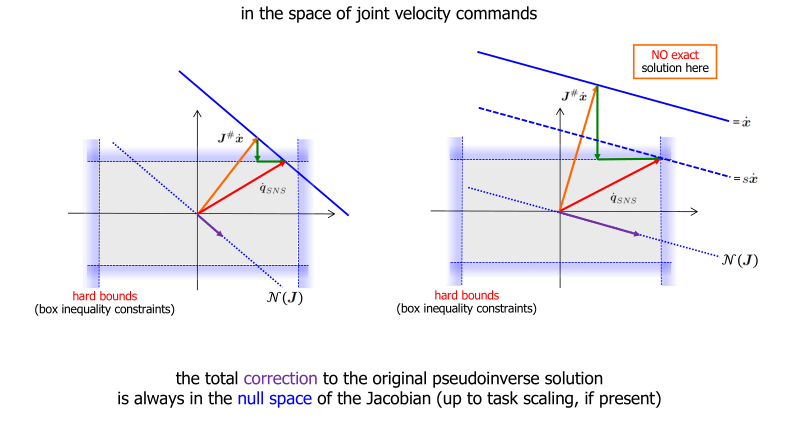
\includegraphics[width=0.8\textwidth]{SNS.png}
\end{figure}

% ---------------------------------------------------------
\subsection{Inclusion of Hard Cartesian Bounds \& Generalized Constraints}
While joint limits are simple "box constraints" ($\dot{q}_{min} \le \dot{q} \le \dot{q}_{max}$), Cartesian limits (like walls, obstacles, or field-of-view restrictions) are \textbf{configuration-dependent}. A joint might be free to rotate, but doing so might push the robot's elbow into a wall. Therefore, these limits must be mapped from the workspace into the joint velocity space.

\textbf{The Concept:} We treat Cartesian boundaries as generalized inequality constraints. When a point on the robot gets too close to a forbidden boundary, we must restrict its velocity \textit{towards} that boundary, while still allowing it to slide parallel to it or move away.

\textbf{Mathematical Formulation \& Calculation of Cartesian Bounds}

\textbf{1. Mapping to Velocity Space:}
Let a Cartesian constraint be defined by a scalar or vector function $c(q)$ (e.g., the distance between the robot and an obstacle). The physical bound is $c(q) \ge c_{min}$. 
Differentiating this with respect to time, we map the limit into the velocity domain using the constraint Jacobian $J_c$:
\begin{equation}
    \dot{c} = J_c(q) \dot{q}
\end{equation}
To ensure the constraint is not violated as the robot approaches the boundary, we enforce an inequality on the velocity:
\begin{equation}
    J_c(q) \dot{q} \ge v_{safe}
\end{equation}
where $v_{safe}$ is typically a function of the distance (e.g., using a potential field or a damping term that forces velocity towards the obstacle to be zero when the distance is critical).

\textbf{2. Calculating $J_c$ via Control Points (Obstacle Avoidance):}
The slides generalize these Cartesian bounds by defining $r$ \textbf{Control Points} along the robot's structure (e.g., the elbow, the end-effector, or any joint that might collide with the environment). If an obstacle is approaching Control Point $r$, we only care about the motion of this specific point. 

The constraint Jacobian $J_c$ in this scenario is simply the \textbf{Geometric Jacobian evaluated at the Control Point $r$} (denoted as $J_r(q)$). To calculate it:
\begin{itemize}
    \item Compute the Jacobian using standard forward kinematics formulas, but \textbf{stop the calculation at the frame of Control Point $r$}, completely ignoring the joints and links that come after it.
    \item If the obstacle only restricts translation (e.g., a wall along the y-axis), you can extract just the relevant linear velocity rows of $J_r(q)$, reducing $J_c$ to a smaller $3 \times n$ (or $1 \times n$) matrix.
\end{itemize}
The Cartesian velocity of the control point is simply $\dot{x}_r = J_r(q) \dot{q}$.

\textbf{3. Unified Treatment in Generalized SNS \& HQP:}
By setting Cartesian box inequalities on the control point's velocity ($\dot{x}_{min} \le J_r(q)\dot{q} \le \dot{x}_{max}$), the problem is formally converted back into the joint velocity domain. 
\begin{itemize}
    \item \textbf{In QP:} These simply become linear inequality constraints of the form $A\dot{q} \le b$, which the solver handles natively.
    \item \textbf{In Generalized SNS:} The algorithm can now process this exactly as it processes joint limits. However, if a Cartesian constraint becomes active, we cannot simply "turn off" a joint with the matrix $W$. Instead, $J_c$ is elevated to the \textbf{highest priority task} (to strictly enforce $\dot{c}_{safe}$).
\end{itemize}

\textbf{4. Sliding on the Boundary (Null-Space Projection):}
If the robot hits a wall, the velocity vector normal to the wall must be zero. However, the robot can still execute its primary task $\dot{x}$ by exploiting the null-space of the constraint Jacobian. The primary task is projected into the null-space of $J_c$:
\begin{equation}
    P_c = I - J_c^\# J_c
\end{equation}
The allowed motion will be forced to "slide" along the Cartesian constraint, completing the primary task only using the degrees of freedom that do not violate the boundary.
% ---------------------------------------------------------
\section{The Dynamic Model}
The goal of the dynamic model is to find the mathematical relationship $\Phi(q, \dot{q}, \ddot{q}) = u$ that links the joint variables (position, velocity, acceleration) to the generalized torques/forces applied to the joints.

\subsection{The Two Problems of Dynamics}
Depending on what is known and what needs to be calculated, we distinguish two main problems:
\begin{itemize}
    \item \textbf{Direct Dynamics (Simulation):} Given the initial state $(q(0), \dot{q}(0))$ and the applied inputs $u(t)$, calculate the resulting motion of the robot $q(t)$.
    \item \textbf{Inverse Dynamics (Control):} Given a desired motion trajectory $(q_d(t), \dot{q}_d(t), \ddot{q}_d(t))$, calculate the required torques/forces $u_d(t)$ that the motors must provide to realize it.
\end{itemize}

\subsection{The Euler-Lagrange Formulation}
Unlike the Newton-Euler method (which is based on force/moment balancing and is highly recursive), the Euler-Lagrange method is an \textbf{energy-based approach}. It is the best method for studying the structural properties of the robot and analyzing control schemes.

\begin{theorybox}{Euler-Lagrange Operational Steps}
\begin{enumerate}
    \item \textbf{Define the Lagrangian ($\mathcal{L}$):} It is defined as the difference between the total Kinetic Energy ($T$) and the total Potential Energy ($U$) of the system:
    \begin{equation}
        \mathcal{L}(q, \dot{q}) = T(q, \dot{q}) - U(q)
    \end{equation}
    
    \item \textbf{Apply the Euler-Lagrange Equation:} For each joint $i$ (from $1$ to $n$), apply the differential operator:
    \begin{equation}
        \frac{d}{dt}\left(\frac{\partial \mathcal{L}}{\partial \dot{q}_i}\right) - \frac{\partial \mathcal{L}}{\partial q_i} = u_i
    \end{equation}
    where $u_i$ is the non-conservative generalized force (e.g., motor torque, friction) performing work on joint $i$.
\end{enumerate}
\end{theorybox}

\subsection{Computing Energies: Kinetic and Potential}
Calculating the energies accurately is the core of most dynamic modeling exercises.

\textbf{1. Kinetic Energy ($T$):}
The total kinetic energy is always described by the quadratic form $T = \frac{1}{2} \dot{q}^T M(q) \dot{q}$, where $M(q)$ is the inertia matrix. To compute it step-by-step for a multi-link robot, we apply \textbf{König's Theorem} link by link:
\begin{equation}
    T = \sum_{i=1}^{n} \left( \frac{1}{2}m_i v_{ci}^T v_{ci} + \frac{1}{2}\omega_i^T I_{ci} \omega_i \right)
\end{equation}
This theorem simply states that the kinetic energy of a rigid body is the sum of the translational energy of its Center of Mass (CoM) and the rotational energy around its CoM. ($v_{ci}$ is the linear velocity of the CoM, $\omega_i$ is the angular velocity, $I_{ci}$ is the barycentric inertia tensor).

\subsubsection*{Rotational Kinetic Energy and Choice of Reference Frame}
In computing the rotational kinetic energy of the $i$-th link, given by the formula:
\begin{equation}
    T_{rot,i} = \frac{1}{2} \boldsymbol{\omega}_i^T \boldsymbol{I}_{c_i} \boldsymbol{\omega}_i
\end{equation}
it is fundamental that the angular velocity vector $\boldsymbol{\omega}_i$ and the barycentric inertia tensor $\boldsymbol{I}_{c_i}$ are expressed in the \textbf{same reference frame} to allow the matrix multiplication.

\textbf{Practical note:} In exercises, it is always convenient to express these quantities in the \textit{link-attached reference frame} (local frame). This way, the inertia matrix $\boldsymbol{I}_{c_i}$ is constant and independent of the robot's configuration.

However, the product $\boldsymbol{\omega}_i^T \boldsymbol{I}_{c_i} \boldsymbol{\omega}_i$ is an \textbf{invariant scalar} with respect to the choice of the reference frame. Being proportional to energy (which is an absolute physical quantity), its value does not change if we change our point of view.

\paragraph*{Proof of Invariance}
If we want to transform from a reference frame $A$ to a frame $B$ through a rotation matrix $\boldsymbol{R}$, we know that:
\begin{itemize}
    \item The angular velocity changes as: $\boldsymbol{\omega}_i^B = \boldsymbol{R} \boldsymbol{\omega}_i^A$
    \item The inertia tensor changes as: $\boldsymbol{I}_{c_i}^B = \boldsymbol{R} \boldsymbol{I}_{c_i}^A \boldsymbol{R}^T$
\end{itemize}

Substituting these expressions into the product computed in frame $B$, we obtain:
\begin{equation}
    (\boldsymbol{\omega}_i^B)^T \boldsymbol{I}_{c_i}^B \boldsymbol{\omega}_i^B = (\boldsymbol{R} \boldsymbol{\omega}_i^A)^T (\boldsymbol{R} \boldsymbol{I}_{c_i}^A \boldsymbol{R}^T) (\boldsymbol{R} \boldsymbol{\omega}_i^A)
\end{equation}

Recalling the transpose property $(\boldsymbol{A}\boldsymbol{B})^T = \boldsymbol{B}^T \boldsymbol{A}^T$:
\begin{equation}
    = (\boldsymbol{\omega}_i^A)^T \boldsymbol{R}^T \boldsymbol{R} \boldsymbol{I}_{c_i}^A \boldsymbol{R}^T \boldsymbol{R} \boldsymbol{\omega}_i^A
\end{equation}

Since the rotation matrix is orthogonal ($\boldsymbol{R}^T \boldsymbol{R} = \boldsymbol{I}$, where $\boldsymbol{I}$ is the identity matrix), the intermediate terms cancel out, yielding:
\begin{equation}
    = (\boldsymbol{\omega}_i^A)^T \boldsymbol{I}_{c_i}^A \boldsymbol{\omega}_i^A
\end{equation}
This demonstrates that the energy value computed in frame $B$ is identical to the one computed in frame $A$.

\vspace{0.5cm}

\textbf{2. Potential Energy ($U$):}
In standard robotics, we generally only consider the contribution of the gravity field. 
\begin{equation}
    U = \sum_{i=1}^{n} U_i \quad \text{with} \quad U_i = -m_i g^T r_{c,i}
\end{equation}
where $r_{c,i}$ is the position vector of the CoM of link $i$, and $g$ is the gravity acceleration vector (e.g., $g = [0, -9.81, 0]^T$).
\begin{examtip}
\textbf{Watch your Kinematics!}\\
As seen in classic exercises (like the Actuated Pendulum or the PR robot), everything relies on properly defining the reference frames and the CoM positions. If you make a mistake in computing $v_{ci}$ or $\omega_i$ (the kinematics), your Kinetic Energy $T$ will be fundamentally flawed, completely compromising the final dynamic equations. \textit{Always double-check your Jacobians and CoM positions first!}
\end{examtip}

\subsection{The Dynamic Model in Matrix Form}
By developing the Euler-Lagrange equations, we obtain the standard vector-matrix form of the dynamic model:
\begin{equation}
    M(q)\ddot{q} + c(q, \dot{q}) + g(q) = u
\end{equation}
You must be able to identify and extract the three main blocks:
\begin{itemize}
    \item \textbf{Inertial Terms ($M(q)\ddot{q}$):} $M(q)$ is the $n \times n$ Inertia Matrix. A crucial property is that $M(q)$ is always \textbf{symmetric and positive definite}, which guarantees it is always invertible.
    
\item \textbf{Coriolis and Centrifugal Terms ($c(q, \dot{q})$):} These terms arise from the kinetic energy derivation and represent the apparent (fictitious) forces acting on the manipulator's links during motion. Since they require non-zero joint velocities ($\dot{q} > 0$), they introduce significant non-linearities and dynamic coupling into the system.
    \begin{itemize}
        \item \textit{Centrifugal effects:} Proportional to squared joint velocities ($\dot{q}_i^2$). Physically, these represent the radial forces that drive the mass of a link outward from its axis of rotation. The joint actuators must generate counteracting torques to resist these outward pulls and maintain structural rigidity along the desired trajectory.
        \item \textit{Coriolis effects:} Proportional to mixed joint velocities ($\dot{q}_i \dot{q}_j$ with $i \neq j$). These effects manifest when a mass moves within a frame of reference that is itself rotating (e.g., the simultaneous rotation of a base joint and the extension of an elbow joint). This combined motion induces transversal forces, causing dynamic cross-coupling where the velocity of one joint directly alters the torque requirements of another.
    \end{itemize}
    While often negligible at low operational speeds—where inertial and gravitational forces dominate—these quadratic velocity terms become highly influential at high speeds. In such regimes, they mandate advanced non-linear control strategies, such as Computed Torque Control (CTC), to actively cancel the dynamic coupling in real-time.
    
    They can be systematically computed using the \textbf{Christoffel Symbols} of the first kind:
    \begin{equation}
        c_{ij}(q) = \frac{1}{2} \left( \frac{\partial M_i}{\partial q_j} + \left(\frac{\partial M_i}{\partial q_j}\right)^T - \frac{\partial M}{\partial q_i} \right)
    \end{equation}
    
    \item \textbf{Gravity Terms ($g(q)$):} These are obtained simply by taking the gradient of the total potential energy with respect to the joint coordinates:
    \begin{equation}
        g(q) = \left( \frac{\partial U}{\partial q} \right)^T
    \end{equation}
\end{itemize}

\subsection{Fundamental Properties of the dynamic model}
The dynamic model exhibits structural properties that are fundamental for control theory and stability proofs. Keep these clearly in mind for theoretical questions:

\begin{enumerate}
    \item \textbf{Skew-Symmetry:} The matrix $\dot{M}(q) - 2C(q,\dot{q})$ is always skew-symmetric, provided that the matrix $C$ is chosen using Christoffel symbols. Mathematically, this means:
    \begin{equation}
        x^T(\dot{M} - 2C)x = 0 \quad \forall x
    \end{equation}
    This property is intimately tied to the conservation of energy and is widely used to prove the asymptotic stability of PD controllers with gravity compensation.
    
    \item \textbf{Conservation of Energy:} If there are no dissipative forces (no friction) and no external active forces performing work ($u \equiv 0$), the total energy of the system $E = T + U$ is strictly conserved. Therefore, its time derivative is zero:
    \begin{equation}
        \dot{E} = 0
    \end{equation}
    \item \textbf{Linear Parameterization:} A fundamental structural property of the rigid robot dynamic model is its linearity with respect to a suitable set of constant dynamic parameters (such as masses, lengths, and inertias). The standard Euler-Lagrange equations can be algebraically rewritten as:
\begin{equation}
    M(q)\ddot{q} + c(q, \dot{q}) + g(q) = Y(q, \dot{q}, \ddot{q}) a = \tau
\end{equation}
where:
\begin{itemize}
    \item $a$ (often also denoted as $\pi$) is a $p$-dimensional vector of \textbf{dynamic coefficients}. These can be the basic parameters (masses, lengths, central inertias) or, more practically, their linear combinations (like the $\rho_k$ coefficients introduced in the 2R planar example).
    \item $Y(q, \dot{q}, \ddot{q})$ is an $n \times p$ matrix known as the \textbf{dynamic regressor}. It is a function solely of the joint positions, velocities, and accelerations, meaning it depends entirely on the kinematics of the manipulator.
\end{itemize}

This linearity property is highly practically relevant, as it forms the mathematical foundation for experimental dynamic parameter identification and the design of adaptive control schemes.
\end{enumerate}

\subsection{Robot Dynamic Model in Vector Formats}

In the study of manipulator dynamics, the equations of motion can be grouped and written in a compact vector form. In general, the implicit form of the model is:
\begin{equation}
    \Phi(q, \dot{q}, \ddot{q}) = u
\end{equation}

\subsubsection{Standard Formulation}
The first form of the dynamic model highlights the individual contributions and is expressed as:
\begin{equation}
    M(q)\ddot{q} + c(q, \dot{q}) + g(q) = u
\end{equation}
where:
\begin{itemize}
    \item $M(q)$ is the inertia matrix, which can be extracted from the kinetic energy $T$ using the Hessian.
    \item $g(q)$ is the vector of gravity terms, calculated as the gradient of the potential energy $U$:
    \begin{equation}
        g(q) = \left( \frac{\partial U}{\partial q} \right)^T
    \end{equation}
    \item $c(q, \dot{q})$ is the vector of Coriolis and centrifugal terms.
\end{itemize}

\paragraph{Coriolis Vector Analysis}
The $k$-th component of the vector $c(q, \dot{q})$ can be rewritten in a quadratic form with respect to the joint velocities:
\begin{equation}
    c_k(q, \dot{q}) = \dot{q}^T C_k(q) \dot{q}
\end{equation}
The associated matrix $C_k(q)$ is defined through the partial derivatives of the inertia matrix:
\begin{equation}
    C_k(q) = \frac{1}{2} \left( \frac{\partial M_k}{\partial q} + \left( \frac{\partial M_k}{\partial q} \right)^T - \frac{\partial M}{\partial q_k} \right)
\end{equation}
where $M_k$ is the $k$-th column of the matrix $M(q)$. It is important to note that, by construction, the matrix $C_k(q)$ is \textbf{symmetric}.

\subsubsection{Factorized Formulation}
It is often very useful, especially for control design, to factorize the Coriolis term by extracting the velocity vector $\dot{q}$. This yields the second form of the model:
\begin{equation}
    M(q)\ddot{q} + C(q, \dot{q})\dot{q} + g(q) = u
\end{equation}

A fundamental note must be made: \textbf{the factorization of vector $c$ is not unique}. This means that $c(q, \dot{q}) = N(q, \dot{q})\dot{q}$ holds true for \textbf{infinite matrices} $N$. 

However, the factorization performed with the matrix $C$ is "special", as the elements of this matrix are obtained using \textbf{Christoffel symbols}:
\begin{equation}
    c_{kj}(q, \dot{q}) = \sum_i c_{kij}(q)\dot{q}_i
\end{equation}
This specific choice preserves important structural properties of the model (such as the skew-symmetry of the matrix $\dot{M} - 2C$).

\subsection{Dynamics of an Actuated Pendulum}

In this section, we analyze the dynamic model of an actuated pendulum as derived using the Euler-Lagrange formulation. We will consider the system generalized coordinate as the link angle $q = \theta$. The motor is connected through a reduction gear with transmission ratio $n_r \ge 1$, so the motor angle is $\theta_m = n_r \theta + \theta_{m0}$ (assuming $\theta_{m0} = 0$).

\begin{figure}[H]
    \centering
    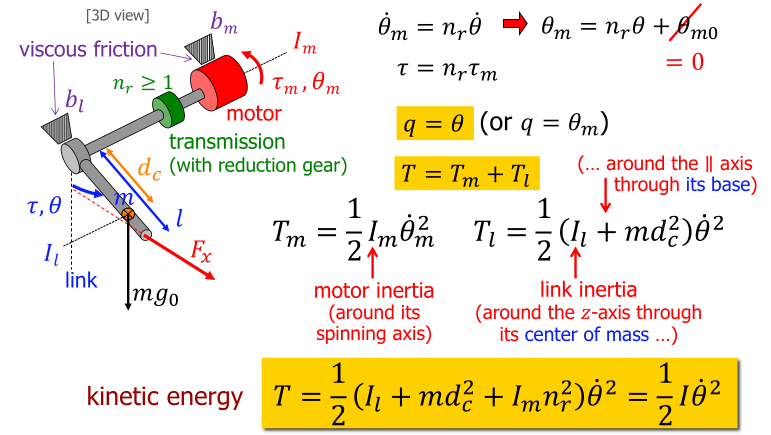
\includegraphics[width=0.8\textwidth]{Pendulum1.png}
\end{figure}

\subsubsection*{Kinetic Energy and the Inertia Question}
The total kinetic energy of the system ($T$) is the sum of the motor's kinetic energy ($T_m$) and the link's kinetic energy ($T_l$):
\begin{equation}
T = T_m + T_l = \frac{1}{2} I_m \dot{\theta}_m^2 + \frac{1}{2} (I_l + m d_c^2) \dot{\theta}^2
\end{equation}
where:
\begin{itemize}
    \item $I_m$ is the motor inertia (around its spinning axis).
    \item $I_l$ is the link inertia around the $z$-axis through its center of mass.
    \item $m$ is the link mass, and $d_c$ is the distance from the joint to the center of mass.
\end{itemize}

\noindent \textbf{The Inertia Question (Parallel Axis / Steiner's Theorem):} 
In the expression for $T_l$, the term $(I_l + m d_c^2)$ represents the equivalent link inertia translated from its center of mass to the parallel axis of rotation at its base. This is a direct application of the parallel axis translation theorem (Steiner's theorem), which states that the moment of inertia around a parallel axis is $I_{zz}' = I_{zz} + m r^2$ (where $r$ is the distance between axes, $d_c$ in this case). 

Substituting $\dot{\theta}_m = n_r \dot{\theta}$, we can express the total kinetic energy purely in terms of the link velocity $\dot{\theta}$:
\begin{equation}
T = \frac{1}{2} (I_l + m d_c^2 + I_m n_r^2) \dot{\theta}^2 = \frac{1}{2} I \dot{\theta}^2
\end{equation}
where $I = I_l + m d_c^2 + I_m n_r^2$ is the total equivalent inertia. Notice that the motor inertia $I_m$ is multiplied by $n_r^2$ when reflected from the motor side to the link side.

\subsubsection*{Potential Energy and Lagrangian}
Assuming gravity $g_0 = 9.81 \text{ m/s}^2$ acts downwards, the potential energy $U$ depends only on the vertical position of the link's center of mass:
\begin{equation}
U = U_0 - m g_0 d_c \cos \theta
\end{equation}
The Lagrangian $L = T - U$ is therefore:
\begin{equation}
L = \frac{1}{2} I \dot{\theta}^2 + m g_0 d_c \cos \theta - U_0
\end{equation}

\subsubsection*{Euler-Lagrange Equations and Generalized Forces}

To find the dynamic equation, we compute the required partial derivatives of the Lagrangian:
\begin{equation}
\frac{\partial L}{\partial \dot{\theta}} = I \dot{\theta} \implies \frac{d}{dt} \left( \frac{\partial L}{\partial \dot{\theta}} \right) = I \ddot{\theta}
\end{equation}
\begin{equation}
\frac{\partial L}{\partial \theta} = - m g_0 d_c \sin \theta
\end{equation}

\begin{figure}[H]
    \centering
    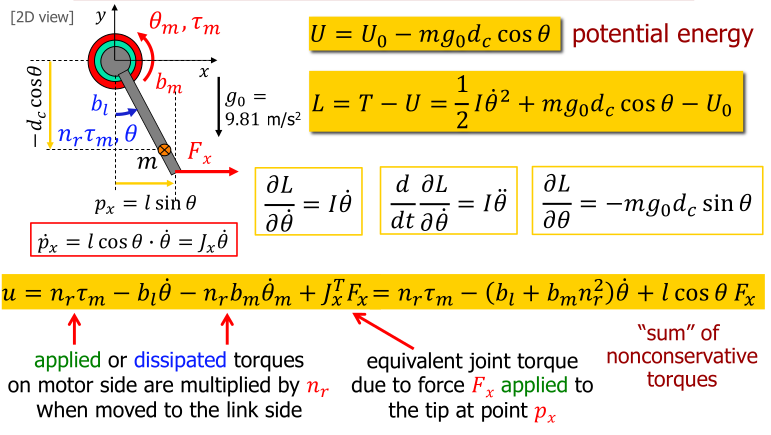
\includegraphics[width=0.8\textwidth]{Pendulum2.png}
\end{figure}


The non-conservative generalized forces $u$ performing work on the coordinate $\theta$ include the equivalent motor torque $\tau$, viscous friction on both the link ($b_l$) and motor ($b_m$), and an external force $F_x$ applied at the tip. The tip position is $p_x = l \sin \theta$, so its velocity is $\dot{p}_x = l \cos \theta \cdot \dot{\theta} = J_x \dot{\theta}$, making the Jacobian $J_x = l \cos \theta$. 

Summing these torques:
\begin{equation}
u = n_r \tau_m - b_l \dot{\theta} - n_r b_m \dot{\theta}_m + J_x^T F_x
\end{equation}
Substituting $\dot{\theta}_m = n_r \dot{\theta}$:
\begin{equation}
u = n_r \tau_m - (b_l + b_m n_r^2) \dot{\theta} + l \cos \theta \cdot F_x
\end{equation}
Notice how the motor friction $b_m$ is also multiplied by $n_r^2$ when moved to the link side, similar to the motor inertia.

\subsubsection*{Final Dynamic Model}
Applying the Euler-Lagrange equation $\frac{d}{dt} \left( \frac{\partial L}{\partial \dot{\theta}} \right) - \frac{\partial L}{\partial \theta} = u$, we obtain the dynamic model in terms of the link coordinate $q = \theta$:
\begin{equation}
I \ddot{\theta} + m g_0 d_c \sin \theta = n_r \tau_m - (b_l + b_m n_r^2) \dot{\theta} + l \cos \theta \cdot F_x
\end{equation}
This scalar equation elegantly captures the inertial, gravitational, and external torque contributions acting on the actuated pendulum system.

\textit{Note: The dynamic model can alternatively be expressed in terms of the motor coordinate $q = \theta_m$ by dividing the entire equation by $n_r$ and substituting $\theta = \theta_m / n_r$.}


% ---------------------------------------------------------
\section{Lagrangian Dynamics}
The dynamic model of a rigid manipulator is derived from the Lagrangian $\mathcal{L}(q, \dot{q}) = T(q, \dot{q}) - U(q)$. The Euler-Lagrange equations yield:
\begin{equation}
    M(q)\ddot{q} + c(q, \dot{q}) + g(q) = \tau
\end{equation}

\subsection{Actuator Dynamics and Friction}
In a real manipulator, torques are provided by motors through reduction gears. If $n_{ri}$ is the gear ratio of the $i$-th joint and $I_{mi}$ is the motor rotor inertia, the kinetic energy of the motors adds a constant diagonal matrix to the inertia matrix:
\begin{equation}
    M_{tot}(q) = M(q) + \text{diag}(n_{ri}^2 I_{mi})
\end{equation}
Additionally, the real torque $\tau$ must compensate for joint friction. The complete model becomes:
\begin{equation}
    M_{tot}(q)\ddot{q} + c(q, \dot{q}) + g(q) + F_v \dot{q} + F_c \text{sgn}(\dot{q}) = \tau
\end{equation}
where $F_v$ is the viscous friction diagonal matrix and $F_c$ is the Coulomb friction diagonal matrix.

\subsection{Link Inertia Matrix and Steiner's Theorem}
In the dynamic modeling of a manipulator, the inertia tensor of a rigid link $i$ is typically known with respect to a frame attached to its center of mass (CoM), denoted as $I_{ci}$. However, for calculating kinetic energy using moving frames, it is often required to express this inertia matrix with respect to a different parallel frame, usually the one attached to the joint origin $O_i$. 

To translate the inertia matrix from the CoM to the joint origin, we apply the \textbf{Steiner's Theorem} (also known as the Parallel Axis Theorem). Let $m_i$ be the mass of the link and $r_{ci} = \begin{bmatrix} x_{c} & y_{c} & z_{c} \end{bmatrix}^T$ be the position vector of the CoM relative to $O_i$. The inertia matrix $I_i$ around the origin $O_i$ is given by:
\begin{equation}
    I_i = I_{ci} + m_i \left( \|r_{ci}\|^2 I_{3\times3} - r_{ci} r_{ci}^T \right)
\end{equation}
where $I_{3\times3}$ is the $3 \times 3$ identity matrix. 
\begin{figure}[H]
    \centering
    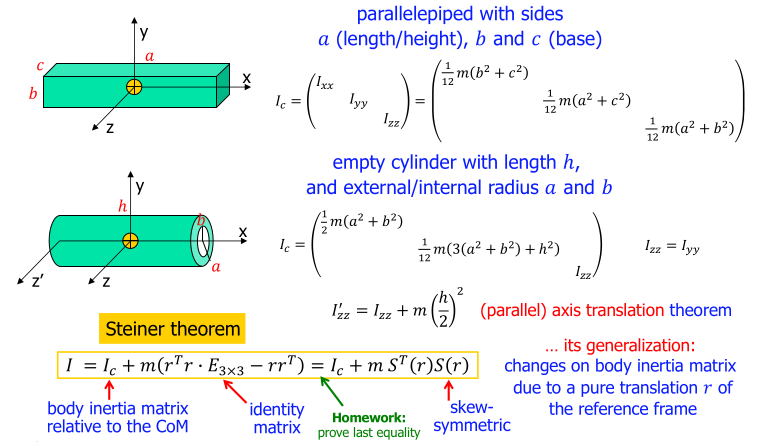
\includegraphics[width=0.8\textwidth]{IntertiasExamples.png}
\end{figure}
Using the skew-symmetric matrix operator $S(\cdot)$ associated with the vector cross product, where $S(r_{ci})v = r_{ci} \times v$, the theorem can be compactly rewritten as:
\begin{equation}
    I_i = I_{ci} - m_i S^2(r_{ci})
\end{equation}
This transformation is essential because, in the moving frames algorithm, all spatial vectors and inertia tensors must be consistently expressed in their respective local coordinate frames to compute the correct kinetic energy terms.

\subsection{Moving Frames Algorithm for Kinetic Energy}
For robots with many degrees of freedom (e.g., $n \ge 4$), calculating the inertia matrix and kinetic energy using standard Jacobians becomes symbolically heavy[cite: 3]. It is therefore useful to operate recursively, expressing each vectorial quantity of link $i$ in its own attached "moving frame" ($RF_i$)[cite: 3]. This approach is particularly convenient when using algebraic or symbolic computation software[cite: 3].

\textbf{Initialization:}
Start from the robot base (link 0) at rest: ${}^0\omega_0 = 0$ and ${}^0v_0 = 0$[cite: 6]. 
Define $\sigma_i = 0$ for a revolute joint and $\sigma_i = 1$ for a prismatic joint[cite: 4].

\textbf{Forward Recursion (from $i=1$ to $n$):}
For each link $i$, calculate the kinematic velocities referenced and projected in the local frame $i$:
\begin{enumerate}
    \item \textbf{Angular velocity of link $i$:}
    \begin{equation}
        {}^i\omega_i = {}^{i-1}R_i^T(q_i) \left[ {}^{i-1}\omega_{i-1} + (1 - \sigma_i) \dot{q}_i \begin{bmatrix} 0 \\ 0 \\ 1 \end{bmatrix} \right]
    \end{equation}
    
    \item \textbf{Linear velocity of the origin $O_i$:}
    \begin{equation}
        {}^iv_i = {}^{i-1}R_i^T(q_i) \left[ {}^{i-1}v_{i-1} + \sigma_i \dot{q}_i \begin{bmatrix} 0 \\ 0 \\ 1 \end{bmatrix} + {}^{i-1}\omega_{i-1} \times {}^{i-1}r_{i-1,i} \right]
    \end{equation}
    
    \item \textbf{Linear velocity of the center of mass (CoM) of link $i$:}
    \begin{equation}
        {}^iv_{ci} = {}^iv_i + {}^i\omega_i \times {}^ir_{ci}
    \end{equation}
\end{enumerate}
\textit{(Note: The equations above assume the standard $z$-axis $[0, 0, 1]^T$ as the joint axis and leverage the already computed vectors from the previous step[cite: 5].)}

\textbf{Total Kinetic Energy Calculation:}
Once all ${}^iv_{ci}$ and ${}^i\omega_i$ are obtained recursively, the total kinetic energy can be written as a sum of local kinetic energies. The main advantage is that the local inertia tensor ${}^iI_i$ is a \textbf{constant matrix} in its moving frame:
\begin{equation}
    T = \sum_{i=1}^n \left( \frac{1}{2}m_i \| {}^iv_{ci} \|^2 + \frac{1}{2} ({}^i\omega_i)^T \, {}^iI_i \, {}^i\omega_i \right)
\end{equation}
From this expression, matching $T = \frac{1}{2} \dot{q}^T M(q) \dot{q}$, the elements of the inertia matrix $M(q)$ can be extracted to compute the Euler-Lagrange equations.

\subsubsection{Center of Mass Position and Asymmetric Mass Distribution}
When defining the dynamic parameters of a link, it is crucial to note that the Center of Mass (CoM) is rarely located at its exact geometric center (e.g., $l_i / 2$). The position vector $r_{ci}$, which locates the CoM relative to the local reference frame $O_i$, depends strictly on the actual mass distribution of the link.
\begin{figure}[H]
    \centering
    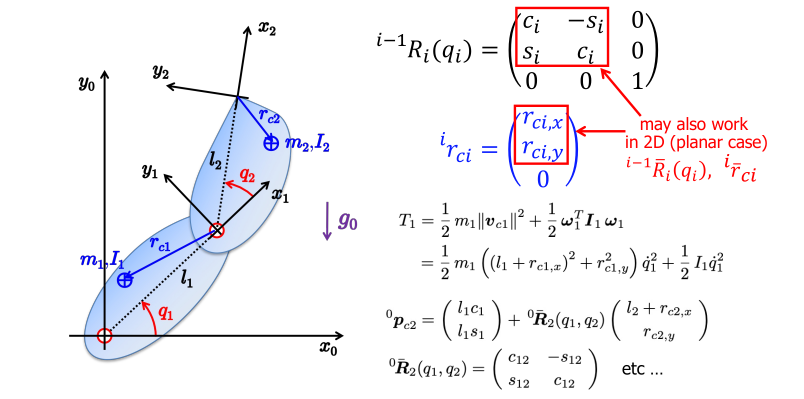
\includegraphics[width=0.8\textwidth]{NotSymmCOM.png}
\end{figure}
In real robotic manipulators, heavy components such as motors, gearboxes, or counterweights are often positioned as close to the base as possible or extending \textit{behind} the joint axis. 

As a result:
\begin{itemize}
    \item The scalar distance identifying the CoM (often denoted as $d_{ci}$) can be negative or result in a vector $r_{ci}$ pointing in the negative direction of the link's longitudinal axis (e.g., $r_{c1,x} = -l_1 + d_{c1}$).
    \item Mechanically, this asymmetry is a deliberate design choice known as \textbf{mass balancing} or \textbf{counterweighting}. 
\end{itemize}
By shifting the CoM backwards toward the preceding joint, the static moment generated by gravity is significantly reduced. This decreases the required holding torque for the previous actuators, thereby improving the overall payload capacity and energy efficiency of the manipulator.



\subsubsection{Step-by-Step Example: Dynamic Model of a 2R Planar Robot}

Consider a 2R planar manipulator moving in the vertical plane, 
with gravity vector $g = \begin{bmatrix} 0 & -g_0 & 0 \end{bmatrix}^T$ where $g_0 = 9.81 \, m/s^2$. 
The assumption is that the center of mass (CoM) of each link lies on its kinematic axis. Let $c_i = \cos(q_i)$, $s_i = \sin(q_i)$, $c_{12} = \cos(q_1+q_2)$, and $s_{12} = \sin(q_1+q_2)$.

\begin{figure}[H]
    \centering
    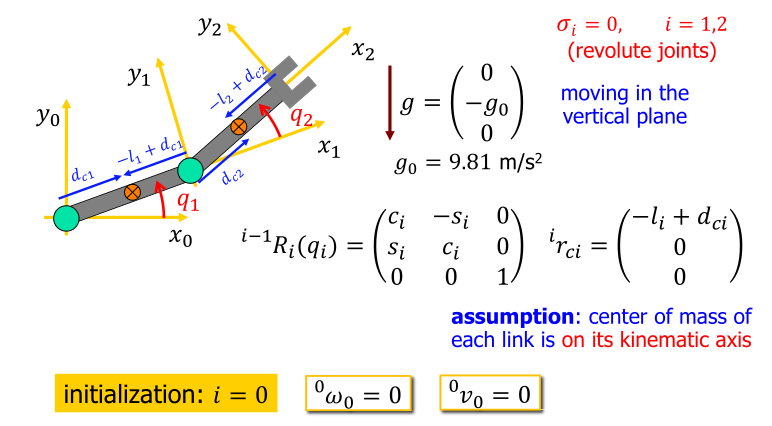
\includegraphics[width=0.8\textwidth]{MovingFrames.png}
\end{figure}

\paragraph{Initialization (Link 0)}
The robot base is at rest:
\begin{equation}
    {}^0\omega_0 = \begin{bmatrix} 0 \\ 0 \\ 0 \end{bmatrix}, \quad {}^0v_0 = \begin{bmatrix} 0 \\ 0 \\ 0 \end{bmatrix}
\end{equation}

\paragraph{First Step (Link 1)}
Applying the forward recursion for $i=1$:
\begin{align}
    {}^1\omega_1 &= {}^0R_1^T(q_1) \left[ {}^0\omega_0 + \dot{q}_1 \begin{bmatrix} 0 \\ 0 \\ 1 \end{bmatrix} \right] = \begin{bmatrix} 0 \\ 0 \\ \dot{q}_1 \end{bmatrix} \\
    {}^1v_1 &= {}^0R_1^T(q_1) \left[ {}^0v_0 + \begin{bmatrix} 0 \\ 0 \\ \dot{q}_1 \end{bmatrix} \times \begin{bmatrix} l_1 c_1 \\ l_1 s_1 \\ 0 \end{bmatrix} \right] = \begin{bmatrix} 0 \\ 0 \\ \dot{q}_1 \end{bmatrix} \times \begin{bmatrix} l_1 \\ 0 \\ 0 \end{bmatrix} = \begin{bmatrix} 0 \\ l_1 \dot{q}_1 \\ 0 \end{bmatrix} \\
    {}^1v_{c1} &= {}^1v_1 + {}^1\omega_1 \times {}^1r_{c1} = \begin{bmatrix} 0 \\ l_1 \dot{q}_1 \\ 0 \end{bmatrix} + \begin{bmatrix} 0 \\ 0 \\ \dot{q}_1 \end{bmatrix} \times \begin{bmatrix} -l_1 + d_{c1} \\ 0 \\ 0 \end{bmatrix} = \begin{bmatrix} 0 \\ d_{c1}\dot{q}_1 \\ 0 \end{bmatrix}
\end{align}
The kinetic energy of link 1 is:
\begin{equation}
    T_1 = \frac{1}{2}m_1 d_{c1}^2 \dot{q}_1^2 + \frac{1}{2}I_{c1,zz}\dot{q}_1^2 = \frac{1}{2}(I_{c1,zz} + m_1 d_{c1}^2)\dot{q}_1^2
\end{equation}

\paragraph{Second Step (Link 2)}
Applying the forward recursion for $i=2$:
\begin{align}
    {}^2\omega_2 &= {}^1R_2^T(q_2) \left[ {}^1\omega_1 + \dot{q}_2 \begin{bmatrix} 0 \\ 0 \\ 1 \end{bmatrix} \right] = \begin{bmatrix} 0 \\ 0 \\ \dot{q}_1 + \dot{q}_2 \end{bmatrix} \\
    {}^2v_2 &= {}^1R_2^T(q_2) \left[ {}^1v_1 + \begin{bmatrix} 0 \\ 0 \\ \dot{q}_1 \end{bmatrix} \times \begin{bmatrix} l_1 \\ 0 \\ 0 \end{bmatrix} \right] = \begin{bmatrix} l_1 s_2 \dot{q}_1 \\ l_1 c_2 \dot{q}_1 + l_2(\dot{q}_1 + \dot{q}_2) \\ 0 \end{bmatrix} \\
    {}^2v_{c2} &= {}^2v_2 + {}^2\omega_2 \times {}^2r_{c2} = \begin{bmatrix} l_1 s_2 \dot{q}_1 \\ l_1 c_2 \dot{q}_1 + d_{c2}(\dot{q}_1 + \dot{q}_2) \\ 0 \end{bmatrix}
\end{align}
The kinetic energy of link 2 is:
\begin{equation}
    T_2 = \frac{1}{2}m_2 \left[ l_1^2 \dot{q}_1^2 + d_{c2}^2(\dot{q}_1 + \dot{q}_2)^2 + 2l_1 d_{c2} c_2 \dot{q}_1(\dot{q}_1 + \dot{q}_2) \right] + \frac{1}{2}I_{c2,zz}(\dot{q}_1 + \dot{q}_2)^2
\end{equation}

\paragraph{Robot Inertia Matrix $M(q)$}
To compactly write $T = T_1 + T_2 = \frac{1}{2} \dot{q}^T M(q) \dot{q}$, we introduce dynamic coefficients $\rho_k$:
\begin{align*}
    \rho_1 &= I_{c1,zz} + m_1 d_{c1}^2 + I_{c2,zz} + m_2 d_{c2}^2 + m_2 l_1^2 \\
    \rho_2 &= m_2 l_1 d_{c2} \\
    \rho_3 &= I_{c2,zz} + m_2 d_{c2}^2 \\
    \rho_4 &= g_0(m_1 d_{c1} + m_2 l_1) \\
    \rho_5 &= g_0 m_2 d_{c2}
\end{align*}
Extracting the matrix terms yields:
\begin{align}
    m_{11}(q) &= \rho_1 + 2\rho_2 \cos(q_2) \\
    m_{12}(q) &= m_{21}(q) = \rho_3 + \rho_2 \cos(q_2) \\
    m_{22}(q) &= \rho_3
\end{align}

\paragraph{Centrifugal and Coriolis Terms $c(q, \dot{q})$}
Using the inertia matrix, the Christoffel symbols approach gives:
\begin{equation}
    c_1(q, \dot{q}) = -\rho_2 s_2 \dot{q}_2^2 - 2\rho_2 s_2 \dot{q}_1 \dot{q}_2, \quad \quad c_2(q, \dot{q}) = \rho_2 s_2 \dot{q}_1^2
\end{equation}

\paragraph{Gravity Terms $g(q)$}
The potential energy is $U = U_1 + U_2 = m_1 g_0 d_{c1} s_1 + m_2 g_0 (l_1 s_1 + d_{c2} s_{12})$. 
Taking the partial derivatives $g(q) = \partial U / \partial q$:
\begin{align}
    g_1(q) &= g_0(m_1 d_{c1} c_1 + m_2 l_1 c_1 + m_2 d_{c2} c_{12}) = \rho_4 c_1 + \rho_5 c_{12} \\
    g_2(q) &= g_0 m_2 d_{c2} c_{12} = \rho_5 c_{12}
\end{align}

\paragraph{Final Dynamic Equations}
Combining all terms into $M(q)\ddot{q} + c(q, \dot{q}) + g(q) = \tau$, the complete model is:
\begin{align}
    \tau_1 &= (\rho_1 + 2\rho_2 c_2)\ddot{q}_1 + (\rho_3 + \rho_2 c_2)\ddot{q}_2 - \rho_2 s_2 \dot{q}_2^2 - 2\rho_2 s_2 \dot{q}_1 \dot{q}_2 + \rho_4 c_1 + \rho_5 c_{12} \\
    \tau_2 &= (\rho_3 + \rho_2 c_2)\ddot{q}_1 + \rho_3 \ddot{q}_2 + \rho_2 s_2 \dot{q}_1^2 + \rho_5 c_{12}
\end{align}

% ---------------------------------------------------------
\section{Dynamic model of robots}

While the Euler-Lagrange formulation provides the base ideal model $M(q)\ddot{q} + c(q,\dot{q}) + g(q) = \tau$, real-world applications and advanced control schemes require understanding the properties, extensions, and task-space mappings of this model.

% --- Bounds on Dynamic Terms ---
\subsection{Bounds on Dynamic Terms}
For an open-chain (serial) manipulator, the dynamic matrices are physically bounded. There always exist positive real constants $k_0$ to $k_7$ such that, for any value of $q$ and $\dot{q}$:
\begin{align}
    k_0 \le \|M(q)\| &\le k_1 + k_2\|q\| + k_3\|q\|^2 \quad &\text{(Inertia matrix)} \\
    \|N(q,\dot{q})\| &\le (k_4 + k_5\|q\|)\|\dot{q}\| \quad &\text{(Coriolis/Centrifugal factorization)} \\
    \|g(q)\| &\le k_6 + k_7\|q\| \quad &\text{(Gravity vector)}
\end{align}
\textbf{Special Case:} If the robot has \textbf{only revolute joints}, the bounds simplify drastically because sines and cosines are naturally bounded between -1 and 1. The limits become independent of the state $q$:
\begin{equation}
    k_0 \le \|M(q)\| \le k_1, \quad \|N(q,\dot{q})\| \le k_4\|\dot{q}\|, \quad \|g(q)\| \le k_6
\end{equation}

% --- Real-World Effects ---
\subsection{Adding Real-World Effects: Actuators, Friction, and Elasticity}
To make the model usable in practice, we must expand the base equation.
\begin{itemize}
    \item \textbf{Friction:} Modeled primarily as Viscous friction $B_v\dot{q}$ (proportional to velocity) and Coulomb friction $B_c\text{sign}(\dot{q})$ (constant, opposes motion direction).
    \item \textbf{Motor Inertia:} The rotor inertia $I_{mi}$ is amplified by the square of the gear reduction ratio $n_{ri}^2$ when reflected to the link side.
\end{itemize}
The complete operational rigid dynamic model becomes:
\begin{equation}
    (M(q) + M_m)\ddot{q} + c(q,\dot{q}) + g(q) + B_v\dot{q} + B_c\text{sign}(\dot{q}) = \tau
\end{equation}
where $M_m = \text{diag}(I_{mi}n_{ri}^2)$.

\textbf{Including Joint Elasticity:} In robots with belts or harmonic drives, joint compliance doubles the generalized coordinates: $n$ link positions ($q$) and $n$ motor positions ($\theta$). The model splits into a $2n$ system:
\begin{align}
    M(q)\ddot{q} + c(q,\dot{q}) + g(q) + K(q - \theta) &= 0 \quad &\text{(Link dynamics)} \\
    M_m\ddot{\theta} + K(\theta - q) &= \tau \quad &\text{(Motor dynamics)}
\end{align}
where $K$ is the diagonal matrix of joint stiffness. External torques $\tau$ only act directly on the motors.

% --- State Space & Linearization ---
\subsection{State Space Representation and Linearization}
For control design and numerical simulation, the second-order model is converted into a \textbf{first-order State Space} model by defining the state vector $x = [q^T, \dot{q}^T]^T \in \mathbb{R}^{2n}$:
\begin{equation}
    \dot{x} = f(x, u) = \begin{bmatrix} \dot{q} \\ M^{-1}(q) [u - c(q, \dot{q}) - g(q)] \end{bmatrix}
\end{equation}
where $u = \tau$ is the input vector.

\begin{theorybox}{Linearization}
To apply linear control techniques, the system is linearized using first-order Taylor expansion around a nominal condition $(x_0, u_0)$, yielding $\delta\dot{x} = A \delta x + B \delta u$, with $A = \frac{\partial f}{\partial x}$ and $B = \frac{\partial f}{\partial u}$.
\begin{itemize}
    \item \textbf{Equilibrium Point (LTI):} If $x_0 = [q_e^T, 0^T]^T$ and $u_0 = g(q_e)$, velocities are zero. Coriolis terms vanish! Matrices $A$ and $B$ are constant:
    \[ A = \begin{bmatrix} 0 & I \\ -M^{-1}(q_e) K_g & 0 \end{bmatrix}, \quad B = \begin{bmatrix} 0 \\ M^{-1}(q_e) \end{bmatrix} \]
    where $K_g = \left. \frac{\partial g(q)}{\partial q} \right|_{q=q_e}$ is the \textbf{gravity stiffness matrix}.
    \item \textbf{Nominal Trajectory (LTV):} If linearized along a moving reference $x_d(t)$, the Jacobians depend on time: $A(t), B(t)$. Coriolis derivatives must be computed.
\end{itemize}
\end{theorybox}

% --- Coordinate Transformation ---
\subsection{Coordinate Transformation}
Given a new set of generalized coordinates $p \in \mathbb{R}^n$ such that $\dot{p} = J(q)\dot{q}$, the dynamic model can be expressed entirely in the new space:
\begin{equation}
    M_p(p)\ddot{p} + c_p(p, \dot{p}) + g_p(p) = u_p
\end{equation}
By applying the principle of virtual work ($u = J^T u_p$) and kinematic differentiation ($\ddot{q} = J^{-1}(\ddot{p} - \dot{J}\dot{q})$), the new terms are:
\begin{align}
    M_p &= J^{-T} M J^{-1} \\
    g_p &= J^{-T} g \\
    c_p &= J^{-T} c - M_p \dot{J} J^{-1} \dot{p}
\end{align}

\begin{examtip}
    Even after coordinate transformation, fundamental structural properties hold! $M_p$ remains symmetric and positive definite (outside singularities), and the matrix $(\dot{M}_p - 2C_p)$ remains \textbf{skew-symmetric}.
\end{examtip}

% --- Task Space & Redundancy ---
\subsection{Task Space Dynamics with Redundancy}
For redundant robots ($m < n$), $J$ is not square. We decompose the joint torques into task-producing torques and null-space torques:
\begin{equation}
    \tau = J^T F + (I - J^T H) \tau_0
\end{equation}

\begin{theorybox}{Dynamically Consistent Inverse}
To prevent internal null-space motions from generating unwanted accelerations at the end-effector ($\ddot{y}$), we choose $H$ as the transpose of the \textbf{inertia-weighted pseudoinverse}:
\begin{equation}
    \bar{J} = M^{-1} J^T (J M^{-1} J^T)^{-1} \implies H = \bar{J}^T
\end{equation}
This perfectly \textit{dynamically decouples} the task dynamics, resulting in:
\begin{equation}
    M_y(q)\ddot{y} + n_y(q, \dot{q}) = F
\end{equation}
where $M_y = (J M^{-1} J^T)^{-1}$ is the \textbf{Task Inertia Matrix}.
\end{theorybox}

% --- Direct vs Inverse Dynamics ---
\subsection{Direct and Inverse Dynamics}
\begin{itemize}
    \item \textbf{Inverse Dynamics (Control/Planning):} Given desired $q, \dot{q}, \ddot{q}$, find the required joint torques $\tau$. Computed algebraically (no integration required).
    \item \textbf{Direct Dynamics (Simulation):} Given current state $q, \dot{q}$ and applied torques $\tau$, find the resulting acceleration $\ddot{q} = M^{-1}(\tau - c - g)$. Requires numerical integration (e.g., Runge-Kutta) to find future states.
\end{itemize}

% --- Dynamic Scaling ---
\subsection{Dynamic Scaling of Trajectories}
If a planned trajectory demands torques exceeding actuator limits ($\tau_{orig}(t) > \tau_{max}$), it is unfeasible. We can recover feasibility by scaling the execution time by a constant factor $k > 1$ (slower execution) without altering the geometric path ($t_{new} = k \cdot t_{old}$).

\begin{recipebox}{Scaling Rules \& Torque Recovery}
Under uniform time scaling by factor $k$:
\begin{itemize}
    \item Position $q$ remains unchanged.
    \item Velocity $\dot{q} \rightarrow \dot{q}/k$.
    \item Acceleration $\ddot{q} \rightarrow \ddot{q}/k^2$.
\end{itemize}
The new required torque scales only in its dynamic components (Inertia and Coriolis). \textbf{Gravity does NOT scale}:
\begin{equation}
    \tau_{new}(kt) = \frac{1}{k^2} \Big( \tau_{orig}(t) - g(q(t)) \Big) + g(q(t))
\end{equation}
\end{recipebox}

\begin{examtip}
    \textbf{Finding the optimal $k^*$ for feasibility:}
    To recover feasibility for a torque limit $\tau_{max}$, isolate the most critical joint $i$ at the most critical time instant $t$, and solve:
    \[ k^* = \max_{i, t} \sqrt{\frac{|\tau_{orig, i}(t) - g_i(q(t))|}{|\tau_{max, i} - g_i(q(t))|}} \]
    \textit{Mandatory Condition:} This is solvable \textbf{only if} $\tau_{max, i} > |g_i(q)| \,\, \forall q$. The actuator must at least be able to support the robot's static weight!
\end{examtip}

% --- Optimal Motion ---
\subsection{Optimal Point-to-Point Robot Motion}
When moving from point A to B, taking the dynamic model into account allows for trajectory optimization:
\begin{itemize}
    \item \textbf{Minimum-Time Motion:} Bang-bang control. At every instant, at least one actuator is saturated at its physical limits. It is the absolute fastest method but causes severe mechanical stress.
    \item \textbf{Minimum-Energy Motion:} Minimizes the integral of squared torques $\int \tau^2 dt$. Produces smoother, harmonious motions, minimizing mechanical wear at the cost of execution time.
\end{itemize}

% ---------------------------------------------------------
\section{Dynamic Redundancy Resolution (LQ Optimization)}
Now we make the final leap. We care not only about \textit{how} the robot moves (accelerations), but \textbf{how much torque/force} the motors must exert to achieve that motion. 

We substitute the joint acceleration $\ddot{q}$ isolated from the dynamic model ($\ddot{q} = M^{-1}(\tau - n(q, \dot{q}))$, where $n = c+g$) into the task kinematic constraint ($J\ddot{q} = \ddot{x}$). 
This yields a \textbf{linear constraint on the torques}:
\begin{equation}
    (J M^{-1}) \tau = \ddot{x} + J M^{-1} n(q, \dot{q})
\end{equation}

Because the robot is redundant, infinite torque vectors $\tau$ satisfy this equation. We find the optimal one by formulating a \textbf{Linear-Quadratic (LQ) Optimization problem}:
Minimize a quadratic cost function $H(\tau) = \frac{1}{2}\tau^T W \tau$ subject to $A\tau = b$.
Using Lagrange multipliers, the universal closed-form solution to this mathematical problem is:
\begin{equation}
    \tau_{opt} = W^{-1} A^T (A W^{-1} A^T)^{-1} b
\end{equation}
where in our robotics context: $A = JM^{-1}$ and $b = \ddot{x} + J M^{-1} n$.

By changing the weight matrix $W$, we obtain the three classic dynamic resolution formulas. Let's see the step-by-step mathematical derivations:

\textbf{Mathematical Proof of the 3 Closed-Form Dynamic Solutions}
\textbf{1. Minimum Torque Norm ($H_1 = \frac{1}{2} \|\tau\|^2$)}
\begin{itemize}
    \item \textbf{Math:} Here there is no weight, so $W = I$ (Identity) and $W^{-1} = I$. Substituting into the general formula:
    $$ \tau_1 = I \cdot A^T (A \cdot I \cdot A^T)^{-1} b = A^T(AA^T)^{-1}b $$
    Notice that $A^T(AA^T)^{-1}$ is the exact definition of the right-pseudoinverse $A^\#$.
    \item \textbf{Solution:} $\tau_1 = (J M^{-1})^\# (\ddot{x} + J M^{-1} n)$
    \item \textbf{Physics:} Minimizes the raw torque effort. It works well for short trajectories but suffers severely from the \textbf{Whipping Effect} on longer paths. Joints accumulate massive internal velocities, causing centrifugal forces to spike, eventually making the required torques explode.
\end{itemize}

\vspace{2mm}
\textbf{2. Minimum Squared Inverse Inertia Weighted ($H_2 = \frac{1}{2} \tau^T M^{-2} \tau$)}
\begin{itemize}
    \item \textbf{Math:} Here $W = M^{-2}$, so $W^{-1} = M^2$. Substituting into the general formula with $A = JM^{-1}$:
    $$ \tau_2 = M^2 (JM^{-1})^T \left[ (JM^{-1}) M^2 (JM^{-1})^T \right]^{-1} b $$
    Since inertia matrices are symmetric, $(M^{-1})^T = M^{-1}$. We can simplify:
    $$ \tau_2 = M^2 M^{-1} J^T \left[ J M^{-1} M^2 M^{-1} J^T \right]^{-1} b $$
    $$ \tau_2 = M J^T \left[ J I J^T \right]^{-1} b = M \underbrace{J^T (J J^T)^{-1}}_{= J^\#} b $$
    \item \textbf{Solution:} $\tau_2 = M J^\# (\ddot{x} + J M^{-1} n)$
    \item \textbf{Physics:} Minimizing this specific weighted torque actually corresponds to \textbf{minimizing the joint accelerations $\ddot{q}$}. This prevents joints from building up crazy internal velocities, neutralizing the whipping effect. This is the recommended, safest approach for general performance.
\end{itemize}

\vspace{2mm}
\textbf{3. Minimum Inverse Inertia Weighted ($H_3 = \frac{1}{2} \tau^T M^{-1} \tau$)}
\begin{itemize}
    \item \textbf{Math:} Here $W = M^{-1}$, so $W^{-1} = M$. Substituting and simplifying:
    $$ \tau_3 = M (JM^{-1})^T \left[ (JM^{-1}) M (JM^{-1})^T \right]^{-1} b $$
    $$ \tau_3 = M M^{-1} J^T \left[ J M^{-1} M M^{-1} J^T \right]^{-1} b $$
    The $M$ and $M^{-1}$ terms cancel out perfectly:
    $$ \tau_3 = J^T \left[ J M^{-1} J^T \right]^{-1} b $$
    \item \textbf{Solution:} $\tau_3 = J^T (J M^{-1} J^T)^{-1} (\ddot{x} + J M^{-1} n)$
    \item \textbf{Physics:} This minimizes the instantaneous \textbf{kinetic energy} associated with the accelerations. The central term $(J M^{-1} J^T)^{-1}$ is the \textbf{Operational Space Inertia Matrix $\Lambda(q)$}. The leading $J^T$ term maps a fictitious Cartesian force directly into joint torques.
\end{itemize}
 

\textbf{Null-Space Damping:} To further stabilize these solutions (especially Case 1 to avoid whipping), we can add an arbitrary torque $\tau_0 = -K_D \dot{q}$ projected into the \textbf{dynamic null space}. This actively dissipates internal kinetic energy, braking the joints without disturbing the end-effector.


\newpage
% ==========================================
% PART 2: HOW TO SOLVE EXERCISES
% ==========================================
\section{How to Solve Midterm Exercises}
\textit{This section provides step-by-step algorithms to solve the exact typologies of exercises found in the exams.}

% ---------------------------------------------------------
\subsection{Type A.1: Task Priority and Task Augmentation}

\textbf{Algorithm: Solving Task Priority (TP) Problems}
\textbf{Goal:} Execute a primary task $\dot{x}_1$ perfectly, and a secondary task $\dot{x}_2$ as best as possible using the remaining degrees of freedom.
\begin{enumerate}
    \item Identify the Jacobians $J_1$ and $J_2$.
    \item Calculate the pseudoinverse of the primary task: $J_1^\# = J_1^T(J_1 J_1^T)^{-1}$.
    \item Calculate the Null-Space projector of the primary task: $P_1 = (I - J_1^\# J_1)$.
    \item The joint velocity for the primary task is: $\dot{q}_1 = J_1^\# \dot{x}_1$.
    \item Calculate the residual error for the second task: $e_2 = \dot{x}_2 - J_2 \dot{q}_1$.
    \item Project $J_2$ into the null space of $J_1$: $\tilde{J}_2 = J_2 P_1$.
    \item The total solution is: $\dot{q}_{TP} = \dot{q}_1 + \tilde{J}_2^\# e_2$.
\end{enumerate}

% ---------------------------------------------------------
\subsubsection{Example: Iterative Task Priority (3 or more tasks)}

 \textbf{Algorithm: General Recursive Formulation (Siciliano-Slotine)}
\textbf{Goal:} Execute multiple tasks strictly ordered by priority (Task 1 $>$ Task 2 $>$ Task 3). This is the exact algorithm to use when handling $N \ge 3$ tasks.
\vspace{0.2cm}

\textbf{1. Initialization:} Start with zero velocity and full available null-space (Identity matrix for an $n$-DOF robot).
\begin{align*}
    P_{A,0} &= I_{n \times n} \\
    \dot{q}_0 &= 0
\end{align*}

\textbf{2. Task 1 (Primary):} Calculate the command for the first task and update the available null-space.
\begin{align*}
    P_{1|0} &= (J_1 P_{A,0})^\# \quad \left[ \text{which simplifies to } J_1^\# \right] \\
    \dot{q}_1 &= \dot{q}_0 + P_{1|0} (\dot{r}_1 - J_1 \dot{q}_0) \quad \left[ \text{which simplifies to } J_1^\# \dot{r}_1 \right] \\
    P_{A,1} &= P_{A,0} - P_{1|0} J_1 P_{A,0} \quad \left[ \text{which simplifies to } I - J_1^\# J_1 \right]
\end{align*}

\textbf{3. Task 2 (Secondary):} Project $J_2$ into the null-space left by Task 1.
\begin{align*}
    P_{2|1} &= (J_2 P_{A,1})^\# \\
    \dot{q}_2 &= \dot{q}_1 + P_{2|1} (\dot{r}_2 - J_2 \dot{q}_1) \\
    P_{A,2} &= P_{A,1} - P_{2|1} J_2 P_{A,1}
\end{align*}

\textbf{4. Task 3 (Tertiary):} Project $J_3$ into the null-space left by Tasks 1 and 2.
\begin{align*}
    P_{3|2} &= (J_3 P_{A,2})^\# \\
    \dot{q}_{TP} &= \dot{q}_2 + P_{3|2} (\dot{r}_3 - J_3 \dot{q}_2)
\end{align*}

\begin{examtip}
\textbf{Pattern Recognition:} Notice the repeating pattern? For any task $k$, you compute the projected inverse $P_{k|k-1}$, update the velocity $\dot{q}_k$ using the error $(\dot{r}_k - J_k \dot{q}_{k-1})$, and finally update the augmented null-space projector $P_{A,k}$. If an exam asks for $4$ tasks, you just add one more block following this exact same logic!
\end{examtip}
\textbf{Algorithm: Solving Task Augmentation (TA) Problems}
\textbf{Goal:} Execute multiple tasks simultaneously by grouping them into a single, higher-dimensional augmented task, treating them with equal priority.
\begin{enumerate}
    \item Identify the Jacobians for the individual tasks: $J_1$ and $J_2$.
    \item Identify the desired velocities for the tasks: $\dot{x}_1$ and $\dot{x}_2$.
    \item Build the \textit{Augmented Jacobian} matrix by stacking the individual Jacobians: 
    \begin{equation*}
        J_A = \begin{bmatrix} J_1 \\ J_2 \end{bmatrix}
    \end{equation*}
    \item Build the \textit{Augmented Task Velocity} vector by stacking the desired velocities: 
    \begin{equation*}
        \dot{x}_A = \begin{bmatrix} \dot{x}_1 \\ \dot{x}_2 \end{bmatrix}
    \end{equation*}
    \item Calculate the pseudoinverse of the Augmented Jacobian: $J_A^\# = J_A^T(J_A J_A^T)^{-1}$ (assuming it has full row rank, otherwise use the general pseudoinverse).
    \item The total joint velocity solution is directly given by: $\dot{q}_{TA} = J_A^\# \dot{x}_A$.
\end{enumerate}

\begin{examtip}
\textbf{Task Priority (TP) vs Task Augmentation (TA):} 
In \textbf{TP}, Task 1 is guaranteed to be executed perfectly (zero tracking error), while Task 2 is executed only in the null-space of Task 1 (it does not interfere). 
In \textbf{TA}, both tasks are forced into one system with equal weight. If the tasks are kinematically incompatible (i.e., they conflict and the robot doesn't have enough DOFs to do both), the pseudoinverse $J_A^\#$ will find a Least Squares solution. This means it will distribute the error between \textit{both} tasks, so neither of them might be perfectly fulfilled!
\end{examtip}


% ---------------------------------------------------------
\subsection{Type A.2: Projected and Reduced Gradient}

 \textbf{Algorithm: Projected Gradient (PG)}
\textbf{Goal:} Execute a task $\dot{x}$ while maximizing/minimizing a scalar objective function $H(q)$.
\begin{enumerate}
    \item Compute the unconstrained solution: $\dot{q}_{task} = J^\# \dot{x}$.
    \item Compute the gradient of your objective function: $\nabla_q H = \begin{bmatrix} \frac{\partial H}{\partial q_1} & \frac{\partial H}{\partial q_2} & \dots \end{bmatrix}^T$.
    \item Define desired null-space velocity: $\dot{q}_0 = \pm \alpha \nabla_q H$ (use $+$ to maximize, $-$ to minimize, with $\alpha > 0$).
    \item Calculate Null-Space projector: $P = (I - J^\# J)$.
    \item Total velocity: $\dot{q}_{PG} = \dot{q}_{task} + P \dot{q}_0$.
\end{enumerate}


 \textbf{Algorithm: Reduced Gradient (RG)}
\textbf{Goal:} Same as PG, but computationally lighter (no pseudoinverse).
\begin{enumerate}
    \item Partition the Jacobian into a square non-singular matrix $J_a$ ($m \times m$) and $J_b$ ($m \times (n-m)$): $J = [J_a \mid J_b]$.
    \item Partition joints accordingly: $q_a$ (dependent) and $q_b$ (independent).
    \item Compute the \textit{Reduced Gradient}: $\nabla_{q_b} H' = [-(J_a^{-1} J_b)^T \mid I] \nabla_q H$.
    \item Update independent joints: $\dot{q}_b = \pm \alpha \nabla_{q_b} H'$.
    \item Solve for dependent joints to ensure task execution: $\dot{q}_a = J_a^{-1}(\dot{x} - J_b \dot{q}_b)$.
\end{enumerate}

\subsubsection{Addendum: Gradient for Obstacle Avoidance}
 \textbf{Algorithm: Maximizing Distance from an Obstacle}
\textbf{Goal:} Calculate the gradient $\nabla_q H$ rapidly when the objective function $H(q)$ is the distance between the robot and a generic obstacle.
\begin{enumerate}
    \item Identify the coordinates of the obstacle $O_m$ and the closest point on the robot $P_m(q)$.
    \item Calculate the unit vector pointing from the obstacle to the robot: $u = \frac{P_m - O_m}{||P_m - O_m||}$.
    \item Compute the Jacobian $J_m(q)$ specifically for the point $P_m$ (NOT the end-effector!).
    \item The gradient is simply: $\nabla_q H = J_m^T(q) u$.
    \item Use this gradient in the standard Projected Gradient (PG) formula.
\end{enumerate}

\vspace{0.3cm}
\noindent \textbf{\large Example: Obstacle Avoidance with PG}
\vspace{0.1cm}

\noindent \textbf{Problem:} The end-effector must execute a velocity task $v_e$, while the robot must maximize its distance from a circular obstacle centered at $O_m$. The closest point on the robot is $P_m$.
\begin{enumerate}
    \item Compute $J_e$ (Jacobian of the end-effector) and $J_m$ (Jacobian of the point $P_m$).
    \item Calculate the task velocity: $\dot{q}_{task} = J_e^\# v_e$.
    \item Calculate the distance gradient: $\nabla_q H_{dist} = J_m^T \frac{P_m - O_m}{||P_m - O_m||}$.
    \item Define the null-space velocity: $\dot{q}_0 = \alpha \nabla_q H_{dist}$ (use positive $\alpha$ to maximize).
    \item Calculate the final command projecting into the null-space of the end-effector:
    $$\dot{q} = \dot{q}_{task} + (I - J_e^\# J_e)\dot{q}_0$$
\end{enumerate}

% ---------------------------------------------------------
\subsection{Type A.3: Singularity Robustness (DLS)}

 \textbf{Algorithm: Damped Least Squares (DLS)}
\textbf{Goal:} Find a safe joint velocity $\dot{q}$ to execute a task $\dot{x}$ when the robot is at or very close to a kinematic singularity, preventing the joint velocities from exploding to infinity.
\begin{enumerate}
    \item Identify the standard task Jacobian $J$.
    \item Choose a damping factor $\lambda > 0$ (often given in the text, or activated only near the singularity).
    \item Calculate the Damped Inverse (Levenberg-Marquardt approach):
    $$J_{DLS} = J^T(JJ^T + \lambda^2 I)^{-1}$$
    \item The joint velocity command is: $\dot{q} = J_{DLS} \dot{x}$.
\end{enumerate}

\vspace{0.3cm}
\noindent \textbf{\large Example: DLS near a Singularity}
\vspace{0.1cm}

\noindent \textbf{Problem:} A planar robot is in an extended singular configuration. A task velocity $\dot{x}$ is commanded along the singular direction (which is physically impossible). Using standard $J^\#$ would result in division by zero. Calculate the DLS velocity.
\begin{enumerate}
    \item Evaluate $J$ at the singular configuration. The matrix $JJ^T$ will have determinant equal to $0$ (it is singular).
    \item Compute $(JJ^T + \lambda^2 I)$. The addition of $\lambda^2$ on the diagonal shifts the eigenvalues, making the matrix strictly positive definite and therefore invertible.
    \item Invert this new regularized matrix.
    \item Multiply by $J^T$ to obtain $J_{DLS}$, and then multiply by the desired task $\dot{x}$:
    $$\dot{q} = J^T(JJ^T + \lambda^2 I)^{-1} \dot{x}$$
    \item \textit{Conceptual Result:} The robot will execute the feasible components of $\dot{x}$ perfectly, while the impossible (singular) components will result in a bounded tracking error instead of causing joint velocities to explode.
\end{enumerate}


% ---------------------------------------------------------
\subsection{Type B: SNS Method (Hard Bounds)}

 \textbf{Algorithm: Saturation in the Null Space (SNS)}
\textbf{Goal:} Find joint velocities that realize the task but strictly respect bounds $|\dot{q}_i| \leq V_{max}$.
\begin{enumerate}
    \item \textbf{Initialize:} Selection matrix $W = I$ (all joints free), saturated velocities $\dot{q}_{sat} = 0$.
    \item \textbf{Compute nominal command:} 
        \begin{itemize}
            \item $a = (JW)^\# \dot{x}$  (Task execution term)
            \item $b = (I - (JW)^\# J)\dot{q}_{sat}$ (Compensation term)
            \item $\dot{q} = a + b$ (Initially, $b=0$ so $\dot{q}=a$)
        \end{itemize}
    \item \textbf{Check bounds:} Does any element of $\dot{q}$ exceed its maximum? If NO, done. If YES, proceed to 4.
    \item \textbf{Saturate worst joint:} Take the joint $k$ that most violates the bound. 
        \begin{itemize}
            \item Set $W_{kk} = 0$ (disable joint $k$).
            \item Set the $k$-th element of $\dot{q}_{sat}$ to $V_{max} \times \text{sign}(\dot{q}_k)$.
        \end{itemize}
    \item \textbf{Re-calculate $a$ and $b$:} Using the updated $W$ and $\dot{q}_{sat}$, recalculate $a = (JW)^\# \dot{x}$ and $b = (I - (JW)^\# J)\dot{q}_{sat}$.
    \item \textbf{Calculate Task Scaling Factor $s$:} To ensure free joints don't violate limits while compensating, find the maximum $s \in [0,1]$ that satisfies for all joints:
    $$ \dot{q}_{min, i} \le s \cdot a_i + b_i \le \dot{q}_{max, i} $$
    \item \textbf{Final command:} Set $\dot{q} = s \cdot a + b$. If bounds are still violated, loop back to step 4 (saturate the next worst joint).
\end{enumerate}


\begin{examtip}
\textbf{The Magic of $a$ and $b$:} Splitting the command into $a$ (task direction) and $b$ (null-space compensation) transforms the highly nonlinear problem of scaling an inverse kinematics solution into a simple linear inequality $s \cdot a_i + b_i$. This makes finding the optimal scale factor $s$ trivial!
\end{examtip}

% ---------------------------------------------------------
\subsection{Type C.1: Deriving the Dynamic Model}

 \textbf{Algorithm: Deriving the Inertia Matrix M}
\textbf{Goal:} Find the symmetric matrix $M(q)$ from kinetic energy $T = \frac{1}{2}\dot{q}^T M(q) \dot{q}$.
\begin{enumerate}
    \item For each link $i$, compute the linear velocity of its Center of Mass, $v_{ci}$, and its angular velocity, $\omega_i$.
    \item \textbf{Planar Robot Shortcut:} $\omega_i$ is simply a scalar on the Z-axis: $\omega_1 = \dot{q}_1$, $\omega_2 = \dot{q}_1 + \dot{q}_2$, etc. $v_{ci} = \frac{d}{dt} p_{ci}(q)$.
    \item Write Kinetic Energy for each link: $T_i = \frac{1}{2}m_i \|v_{ci}\|^2 + \frac{1}{2}\omega_i^T I_{ci} \omega_i$.
    \item Sum them up: $T_{tot} = \sum T_i$.
    \item Expand $T_{tot}$ and group terms into the quadratic form $\frac{1}{2} \sum \sum m_{ij}(q)\dot{q}_i \dot{q}_j$. The coefficients form $M(q)$.
\end{enumerate}


 \textbf{Algorithm: Deriving Coriolis and Centrifugal terms c}
\textbf{Method: Christoffel Symbols (Fast Matrix form)}
Let $M_k$ be the $k$-th column of $M(q)$. The $k$-th element of vector $c$ is $c_k = \dot{q}^T C_k(q) \dot{q}$, where:
\begin{equation}
    C_k(q) = \frac{1}{2} \left[ \frac{\partial M_k}{\partial q} + \left(\frac{\partial M_k}{\partial q}\right)^T - \frac{\partial M}{\partial q_k} \right]
\end{equation}
Stack the resulting scalars to get the vector $c(q, \dot{q})$.
 \

 \textbf{Algorithm: Deriving Gravity Vector g}
\begin{enumerate}
    \item Find the height $y_{ci}$ (component aligned with gravity vector) of each CoM.
    \item Write total potential energy: $U(q) = \sum m_i g_0 y_{ci}$.
    \item Differentiate: $g(q) = \left( \frac{\partial U(q)}{\partial q} \right)^T$.
\end{enumerate}

% ---------------------------------------------------------
\subsection{Type C.2: Inverse Dynamics}

 \textbf{Algorithm: Computing Inverse Dynamics Torque}
\textbf{Goal:} Calculate the required joint torques $\tau_d(t)$ to perfectly track a given desired trajectory $q_d(t)$.
\begin{enumerate}
    \item \textbf{Derive Trajectory:} Given $q_d(t)$, compute its first derivative $\dot{q}_d(t)$ (velocity) and second derivative $\ddot{q}_d(t)$ (acceleration).
    \item \textbf{Substitute into Model:} Take the symbolic dynamic model you found: $M(q)\ddot{q} + c(q,\dot{q}) + g(q) = \tau$.
    \item \textbf{Evaluate:} Substitute $q = q_d(t)$, $\dot{q} = \dot{q}_d(t)$, and $\ddot{q} = \ddot{q}_d(t)$ into the equations.
    \item \textbf{Alternative via Regressor:} If you have already computed the regressor $Y$ and parameters $\mathbf{a}$, you can simply compute $\tau_d(t) = Y(q_d, \dot{q}_d, \ddot{q}_d)\mathbf{a}$. This is often much faster and less prone to algebraic errors!
\end{enumerate}

% ---------------------------------------------------------
\subsubsection{Example: Computing Inverse Dynamics via Regressor}

 \textbf{Problem:} Given the linear parameterization $Y(q, \dot{q}, \ddot{q})\mathbf{a} = \tau$ and a desired trajectory $q_d(t) = \begin{bmatrix} A \sin(\omega t) \\ B \cos(\omega t) \end{bmatrix}$, find the required joint torques $\tau_d(t)$.
\vspace{0.2cm}

\textbf{1. Calculate velocity and acceleration:}
\begin{align*}
    \dot{q}_d(t) &= \begin{bmatrix} A \omega \cos(\omega t) \\ -B \omega \sin(\omega t) \end{bmatrix} \\
    \ddot{q}_d(t) &= \begin{bmatrix} -A \omega^2 \sin(\omega t) \\ -B \omega^2 \cos(\omega t) \end{bmatrix}
\end{align*}

\textbf{2. Evaluate the Regressor Matrix:} 
Substitute $q_d(t)$, $\dot{q}_d(t)$, and $\ddot{q}_d(t)$ into your previously found symbolic matrix $Y(q, \dot{q}, \ddot{q})$ to obtain the time-dependent matrix $Y_d(t)$.
\begin{equation*}
    Y_d(t) = Y(q_d(t), \dot{q}_d(t), \ddot{q}_d(t))
\end{equation*}

\textbf{3. Compute the torques:} 
Multiply the evaluated regressor by your vector of constant dynamic parameters $\mathbf{a}$ (which contains grouped terms like $m_1, I_1, m_2, I_2$).
\begin{equation*}
    \tau_d(t) = Y_d(t) \mathbf{a}
\end{equation*}

% ---------------------------------------------------------
\textbf{\large Full Procedure for Linear Parameterization and Inverse Dynamics}

\textbf{Problem:} Extract the regressor $Y$, the parameter vector $\mathbf{a}$, and compute the inverse dynamics torque $\tau_d(t)$ for a given trajectory $q_d(t)$.
\vspace{0.2cm}

\textbf{1. Expand the Dynamic Model:}
Write out the full equations of motion for each joint ($\tau_1, \tau_2, \dots$) by expanding $M(q)\ddot{q} + c(q,\dot{q}) + g(q)$. For example, a generic first joint equation might look like:
\begin{equation*}
    \tau_1 = (I_1 + m_1 l_{c1}^2 + m_2 l_1^2)\ddot{q}_1 + (I_2 + m_2 l_{c2}^2)(\ddot{q}_1 + \ddot{q}_2) + m_2 l_1 l_{c2} \cos(q_2)(2\ddot{q}_1 + \ddot{q}_2) + \dots
\end{equation*}

\textbf{2. Define the Parameter Vector $\mathbf{a}$:}
Identify the constant physical parameters (masses, inertias, lengths) that always appear grouped together. Define them as a new set of coefficients $a_i$.
\begin{align*}
    a_1 &= I_1 + m_1 l_{c1}^2 + m_2 l_1^2 \\
    a_2 &= I_2 + m_2 l_{c2}^2 \\
    a_3 &= m_2 l_1 l_{c2}
\end{align*}
So, your parameter vector is $\mathbf{a} = \begin{bmatrix} a_1 & a_2 & a_3 \end{bmatrix}^T$.

\textbf{3. Build the Regressor Matrix $Y(q, \dot{q}, \ddot{q})$:}
The Regressor Matrix $Y$ is an $n \times p$ matrix (number of joints $\times$ number of dynamic parameters) that contains exclusively the kinematic variables ($q, \dot{q}, \ddot{q}$) and the gravity constant $g_0$. It separates the motion from the mass/inertia properties.

\textbf{How to construct it row by row:}
\begin{itemize}
    \item Look at the equation for $\tau_1$ (which corresponds to \textbf{Row 1} of $Y$).
    \item Ask yourself: \textit{"What multiplies $a_1$?"} The answer is $\ddot{q}_1$. This goes into position $Y_{1,1}$.
    \item Ask yourself: \textit{"What multiplies $a_2$?"} The answer is $(\ddot{q}_1 + \ddot{q}_2)$. This goes into position $Y_{1,2}$.
    \item Repeat this process for the equation of $\tau_2$ (\textbf{Row 2} of $Y$). If a parameter $a_i$ does not appear in the equation for a specific joint, simply place a $0$ in that column (e.g., $a_1$ does not appear in $\tau_2$, so $Y_{2,1} = 0$).
\end{itemize}

Applying this logic, we factor out the vector $\mathbf{a}$ and obtain:
\begin{equation*}
    \begin{bmatrix} \tau_1 \\ \tau_2 \end{bmatrix} =
    \underbrace{\begin{bmatrix}
        \ddot{q}_1 & \ddot{q}_1 + \ddot{q}_2 & \cos(q_2)(2\ddot{q}_1 + \ddot{q}_2) - \sin(q_2)(2\dot{q}_1\dot{q}_2 + \dot{q}_2^2) \\
        0 & \ddot{q}_1 + \ddot{q}_2 & \cos(q_2)\ddot{q}_1 + \sin(q_2)\dot{q}_1^2
    \end{bmatrix}}_{Y(q, \dot{q}, \ddot{q})}
    \underbrace{\begin{bmatrix} a_1 \\ a_2 \\ a_3 \end{bmatrix}}_{\mathbf{a}}
\end{equation*}
This $2 \times 3$ matrix is your Regressor $Y(q, \dot{q}, \ddot{q})$.

\textbf{4. Compute Inverse Dynamics Torques $\tau_d(t)$:}
Given a desired trajectory, e.g., $q_d(t) = \begin{bmatrix} A \sin(\omega t) \\ B \cos(\omega t) \end{bmatrix}$:
\begin{itemize}
    \item Compute velocities $\dot{q}_d(t)$ and accelerations $\ddot{q}_d(t)$ by taking the 1st and 2nd time derivatives of $q_d(t)$.
    \item Substitute $q_d, \dot{q}_d, \ddot{q}_d$ directly into the matrix $Y$ to obtain the time-dependent matrix $Y_d(t)$.
    \item Multiply by the constant vector $\mathbf{a}$ to get the required torques.
\end{itemize}
\begin{equation*}
    \tau_d(t) = Y_d(t) \mathbf{a}
\end{equation*}

\textit{Note: Doing $\tau_d(t) = Y_d(t) \mathbf{a}$ directly outputs the torques without needing to re-evaluate the heavy $M$, $c$, and $g$ matrices individually, saving significant time during the exam.}
% ---------------------------------------------------------
\subsection{Type D: Skew-Symmetry and Factorizations}

 \textbf{Algorithm: Finding Factorizations S1 and S2}
\textbf{Goal:} Find matrices $S$ such that $S \dot{q} = c$, one making $\dot{M} - 2S$ skew-symmetric ($S_1$), and one not ($S_2$).
\begin{enumerate}
    \item \textbf{Skew-symmetric $S_1$:} Stack the Christoffel matrices you found earlier!
    \begin{equation}
        S_1(q,\dot{q}) = \begin{bmatrix} \dot{q}^T C_1(q) \\ \dot{q}^T C_2(q) \\ \dots \end{bmatrix}
    \end{equation}
    
    \item \textbf{NON skew-symmetric $S_2$:} 
    Add a dummy matrix $S_0(\dot{q})$ to $S_1$ such that $S_0(\dot{q})\dot{q} = 0$. For a 2-DOF robot, choose:
    $$ S_0(\dot{q}) = \begin{bmatrix} 0 & -\dot{q}_2 \\ \dot{q}_2 & 0 \end{bmatrix} $$
    Then $S_2 = S_1 + S_0$. Since $S_0 \dot{q} = 0$, $S_2 \dot{q} = c(q, \dot{q})$, but $\dot{M}-2S_2$ will NOT be skew-symmetric.
\end{enumerate}
% ---------------------------------------------------------
\subsection{Type E: Linear Parameterization and Identification}

 \textbf{Algorithm: Extracting Regressor Y and parameters a}
\textbf{Goal:} Rewrite $M\ddot{q} + c + g = \tau$ as $Y(q, \dot{q}, \ddot{q})\mathbf{a} = \tau$.
\begin{enumerate}
    \item Identify all blocks of constants (masses, lengths, inertias). Group terms that always appear together (e.g., $I_1 + m_1 l_{c1}^2$) into a single dynamic coefficient $a_k$.
    \item Define your vector $\mathbf{a} = [a_1, a_2, \dots, a_p]^T$.
    \item Rewrite the equations of motion isolating the variables.
    \item Extract the variables into the $n \times p$ matrix $Y$. 
\end{enumerate}


 \textbf{Algorithm: Dynamic Identification}
Once you have $Y\mathbf{a} = \tau$, to find the true parameters $\mathbf{a}$ experimentally:
\begin{enumerate}
    \item Sample $q, \dot{q}, \ddot{q}$ and $\tau$ at $N$ time instants along an exciting trajectory.
    \item Build the stacked Regressor Matrix $\bar{Y}$ ($nN \times p$) and Torque vector $\bar{\tau}$ ($nN \times 1$).
    \item Solve using Least Squares: $\hat{\mathbf{a}} = \bar{Y}^\# \bar{\tau} = (\bar{Y}^T \bar{Y})^{-1} \bar{Y}^T \bar{\tau}$.
\end{enumerate}
% ---------------------------------------------------------
\subsection{Type F: Dynamic Redundancy Resolution (LQ Opt.)}

 \textbf{Algorithm: Solving LQ Dynamic Redundancy}
\textbf{Goal:} Find the joint torque $\tau$ that executes a Cartesian task $\ddot{y}$ while minimizing a specific physical effort $H(\tau)$.
\begin{enumerate}
    \item Isolate the "clean" task acceleration: $\ddot{x} = \ddot{y} - \dot{J}\dot{q}$.
    \item Group the dynamic bias terms: $n(q,\dot{q}) = c(q,\dot{q}) + g(q)$.
    \item Define the constant vector $b = \ddot{x} + J M^{-1}n$.
    \item Apply the correct closed-form solution based on the text's request:
    \begin{itemize}
        \item \textbf{Min $\| \tau \|^2$}: $\tau_1 = (J M^{-1})^\# b$.
        \item \textbf{Min $\| \tau \|^2_{M^{-2}}$}: $\tau_2 = M J^\# b$.
        \item \textbf{Min $\| \tau \|^2_{M^{-1}}$}: $\tau_3 = J^T (J M^{-1} J^T)^{-1} b$.
    \end{itemize}
\end{enumerate}
% ---------------------------------------------------------
\subsection{Type G: Time Scaling under Torque Bounds}

 \textbf{Algorithm: Uniform Time Scaling}
\textbf{Goal:} Find scale factor $k \ge 1$ to satisfy torque bounds $|u_i| \le U_{max}$ without altering the geometric path.
\begin{enumerate}
    \item Determine the max required torque $\tau_{orig}(t)$ during the given trajectory using Inverse Dynamics.
    \item Separate the torque into Gravity terms ($g$) which DO NOT scale, and Inertial/Coriolis terms ($\tau_{dyn}$) which scale with $1/k^2$.
    \item Set up the inequality for the most critical joint:
    \begin{equation}
        \left| \frac{\tau_{dyn}}{k^2} + g \right| \leq U_{max}
    \end{equation}
    \item Solve for $k$:
    \begin{equation}
        k \geq \sqrt{\frac{|\tau_{dyn}|}{U_{max} - |g|}}
    \end{equation}
    \item The new feasible execution time is $T_s = k \cdot T_{old}$.
\end{enumerate}


\subsection{Type H: Energy Dissipation and Optimal Torque Selection}
\textbf{Problem:} Given the bounds on joint torques $|\tau_j| \le T_j$, determine the commanded torque $\tau$ that maximizes the instantaneous decrease of the total energy $E = T + U$ of the robot.

\textbf{Algorithm: Maximizing Energy Decrease} \\
\textbf{Goal:} Choose the joint torques $\tau$ to make the energy time derivative $\dot{E}$ (or its second derivative $\ddot{E}$ if the robot is completely at rest) as negative as possible.

\begin{enumerate}
    \item \textbf{Case 1: The robot is currently in motion ($\dot{q} \neq 0$)}
    \begin{itemize}
        \item Start from the power/energy variation formula: 
        \begin{equation}
            \dot{E} = \dot{q}^T \tau = \sum_{j=1}^n \dot{q}_j \tau_j
        \end{equation}
        \item To make $\dot{E}$ as negative as possible, apply the maximum available torque in the exact \emph{opposite} direction of the current velocity. For each joint $j$ where $\dot{q}_j \neq 0$, set:
        \begin{equation}
            \tau_{0,j} = -T_j \text{sign}(\dot{q}_j)
        \end{equation}
        \item If a joint is not moving ($\dot{q}_j = 0$), its torque does not contribute to $\dot{E}$ in this instant, so you can simply command $\tau_{0,j} = 0$.
        \item The resulting guaranteed maximum energy decrease is:
        \begin{equation}
            \dot{E}_{max} = -\sum_{\dot{q}_j \neq 0} T_j |\dot{q}_j| < 0
        \end{equation}
    \end{itemize}

    \item \textbf{Case 2: The robot is at rest ($\dot{q} = 0$) but not in equilibrium ($g(q_0) \neq 0$)}
    \begin{itemize}
        \item Since $\dot{q} = 0$, the first derivative is strictly zero: $\dot{E} = 0$ regardless of the torque chosen. To induce a decrease in the immediate future, we must force the second derivative $\ddot{E}$ to be negative.
        \item Differentiate $\dot{E}$: $\ddot{E} = \ddot{q}^T \tau + \dot{q}^T \dot{\tau}$. Since $\dot{q} = 0$, it simplifies to:
        \begin{equation}
            \ddot{E} = \ddot{q}^T \tau
        \end{equation}
        \item Use the standard dynamic model $M(q)\ddot{q} + c(q,\dot{q}) + g(q) = \tau$. At $\dot{q}=0$, the Coriolis terms vanish ($c(q_0,0)=0$). Isolate the joint acceleration $\ddot{q}$:
        \begin{equation}
            \ddot{q} = M^{-1}(q_0)(\tau - g(q_0))
        \end{equation}
        \item Substitute $\ddot{q}$ into $\ddot{E}$ to obtain a complete quadratic function of the variable $\tau$:
        \begin{equation}
            \ddot{E}(\tau) = \tau^T M^{-1}(q_0) \tau - g^T(q_0) M^{-1}(q_0) \tau
        \end{equation}
        \item Find the theoretical minimum by taking the gradient of $\ddot{E}$ with respect to $\tau$ and setting it to zero:
        \begin{equation}
            \nabla_{\tau}\ddot{E} = 2 M^{-1}(q_0) \tau - M^{-1}(q_0) g(q_0) = \mathbf{0}
        \end{equation}
        \item Since $M^{-1}(q_0)$ is a positive definite (and therefore invertible) matrix, we can cleanly solve for $\tau$. The unique optimal torque to immediately dissipate energy is exactly half the gravity compensation vector:
        \begin{equation}
            \tau_{0} = \frac{g(q_0)}{2}
        \end{equation}
        \item \emph{Final Verification:} The Hessian matrix is $\nabla^2_{\tau}\ddot{E} = 2M^{-1}(q_0) > 0$, guaranteeing this is a global minimum. Evaluating the function yields a strictly negative energy acceleration:
        \begin{equation}
            \ddot{E}(\tau_0) = -\frac{1}{4} g^T(q_0) M^{-1}(q_0) g(q_0) < 0
        \end{equation}
    \end{itemize}
\end{enumerate}

\subsubsection*{Deep Dive: Mathematical Proof for Case 2 ($\dot{q} = 0$)}
To rigorously prove why $\tau_0 = \frac{g(q_0)}{2}$ minimizes the energy acceleration $\ddot{E}$, we can analyze the individual contributions of the kinetic energy $T$ and potential energy $U$.

\textbf{0. Base Energy Definitions}
\begin{itemize}
    \item \textbf{Kinetic Energy:} $T(q, \dot{q}) = \frac{1}{2} \dot{q}^T M(q) \dot{q}$
    \item \textbf{Potential Energy:} $U(q)$, whose gradient with respect to $q$ is the gravity vector: $\frac{\partial U}{\partial q} = g^T(q)$
\end{itemize}

\textbf{1. Joint Acceleration Mapping} \\
Starting from the dynamic model at rest ($\dot{q} = 0$, so the Coriolis/centrifugal terms $c(q_0, 0) = \mathbf{0}$):
\begin{equation}
    M(q_0)\ddot{q} + g(q_0) = \tau
\end{equation}
Substituting our optimal torque $\tau = \frac{g(q_0)}{2}$ and solving for $\ddot{q}$:
\begin{equation}
    M(q_0)\ddot{q} = -\frac{1}{2}g(q_0) \implies \ddot{q} = -\frac{1}{2}M^{-1}(q_0)g(q_0)
\end{equation}

\textbf{2. Kinetic Energy Derivatives ($T$)}
\begin{itemize}
    \item $T = 0$ (since the robot is at rest, $\dot{q} = 0$).
    \item $\dot{T} = 0$ (the net power depends linearly on $\dot{q}$, so it vanishes).
    \item For $\ddot{T}$, evaluating the second time derivative at $\dot{q} = 0$ eliminates all complex velocity-dependent terms, leaving only the acceleration quadratic form:
    \begin{equation}
        \ddot{T} = \ddot{q}^T M(q_0) \ddot{q}
    \end{equation}
    Substituting $\ddot{q}$ from step 1 (and knowing $M^{-1}$ is symmetric):
    \begin{equation}
        \ddot{T} = \left(-\frac{1}{2}g^T M^{-1}\right) M \left(-\frac{1}{2}M^{-1}g\right) = \frac{1}{4}g^T M^{-1} g > 0
    \end{equation}
\end{itemize}

\textbf{3. Potential Energy Derivatives ($U$)}
\begin{itemize}
    \item $U = U(q_0) \ge 0$
    \item $\dot{U} = g^T(q) \dot{q} = 0$ (since $\dot{q} = 0$).
    \item For $\ddot{U}$, taking the time derivative of $\dot{U}$ yields $\ddot{U} = \dot{q}^T \frac{\partial g}{\partial q} \dot{q} + g^T \ddot{q}$. At $\dot{q}=0$, the first term vanishes:
    \begin{equation}
        \ddot{U} = g^T(q_0) \ddot{q}
    \end{equation}
    Substituting $\ddot{q}$ from step 1:
    \begin{equation}
        \ddot{U} = g^T(q_0) \left(-\frac{1}{2}M^{-1}(q_0)g(q_0)\right) = -\frac{1}{2}g^T M^{-1} g < 0
    \end{equation}
\end{itemize}

\textbf{4. Total Energy Balance ($E$)} \\
Summing the derived second derivatives gives the total energy acceleration:
\begin{equation}
    \ddot{E} = \ddot{T} + \ddot{U} = \frac{1}{4}g^T M^{-1} g - \frac{1}{2}g^T M^{-1} g = -\frac{1}{4}g^T M^{-1} g < 0
\end{equation}

\textit{Physical insight:} Applying exactly half the required gravity compensation torque allows the robot to "fall" slightly, which immediately decreases its potential energy ($\ddot{U} < 0$) while it starts gaining some kinetic energy ($\ddot{T} > 0$). The mathematical catch is that the potential energy decreases exactly \emph{twice as fast} as the kinetic energy increases, resulting in the maximum possible net instantaneous dissipation of the total energy $E$.

\newpage
% ==========================================
% PART 3: PROOFS
% ==========================================

\section{Proofs}

\subsection{Minimum Norm Solution for Kinematic Redundancy}
\textbf{Theorem:} Given a redundant manipulator with differential kinematic equation $\dot{y} = J(q)\dot{q}$, where $J$ has full row rank. Among all possible joint velocity solutions $\dot{q}$ that satisfy the task constraint, the one minimizing the quadratic norm of the joint velocities $\frac{1}{2} \|\dot{q}\|^2$ is given by $\dot{q} = J^\# \dot{y}$, where $J^\# = J^T(JJ^T)^{-1}$ is the Moore-Penrose right pseudoinverse.

\subsubsection{Proof}
We can find the solution by formulating a constrained optimization problem using Lagrange multipliers.
The Lagrangian function is defined as:
\[
L(\dot{q}, \lambda) = \frac{1}{2} \dot{q}^T \dot{q} + \lambda^T (\dot{y} - J \dot{q})
\]
where $\lambda$ is the vector of Lagrange multipliers. 
We compute the partial derivatives with respect to $\dot{q}$ and set them to zero to find the stationary point:
\[
\frac{\partial L}{\partial \dot{q}} = \dot{q}^T - \lambda^T J = 0 \implies \dot{q} = J^T \lambda
\]
Substituting this expression for $\dot{q}$ back into the original task constraint $\dot{y} = J\dot{q}$:
\[
\dot{y} = J (J^T \lambda) = (J J^T) \lambda
\]
Since $J$ has full row rank, the square matrix $(J J^T)$ is strictly positive definite and therefore invertible. We can solve for $\lambda$:
\[
\lambda = (J J^T)^{-1} \dot{y}
\]
Finally, substituting $\lambda$ into the expression for $\dot{q}$, we obtain the proof:
\[
\dot{q} = J^T (J J^T)^{-1} \dot{y} = J^\# \dot{y}
\]


\subsection{Null-Space Projection Matrix (Task Priority)}
\textbf{Property:} The matrix $P(q) = I - J^\#(q)J(q)$ is an orthogonal projector that maps any arbitrary joint velocity vector $\dot{q}_0$ into the null-space of the Jacobian $J$, meaning it does not alter the execution of the primary task.

\subsubsection{Proof}
To prove that $P$ projects into the null-space of $J$, we must verify that the contribution of $P \dot{q}_0$ to the task $\dot{y}$ is strictly zero. We multiply the projector by the Jacobian matrix $J$:
\[
J P = J (I - J^\# J) = J - J J^\# J
\]
Substituting the definition of the right pseudoinverse $J^\# = J^T(JJ^T)^{-1}$:
\[
J J^\# J = J \left[ J^T(JJ^T)^{-1} \right] J = (JJ^T)(JJ^T)^{-1}J = I \cdot J = J
\]
Therefore:
\[
J P = J - J = 0
\]
Furthermore, an orthogonal projector must be idempotent ($P^2 = P$) and symmetric ($P^T = P$).
Proving idempotence:
\[
P^2 = (I - J^\# J)(I - J^\# J) = I - 2J^\# J + J^\# J J^\# J = I - 2J^\# J + J^\# J = I - J^\# J = P
\]


\subsection{Linearization for Kinematic Calibration}
\textbf{Derivation:} To identify the kinematic parameters (e.g., Denavit-Hartenberg parameters $\pi$), an iterative least-squares approach is used based on the first-order linearization of the direct kinematics equation.

\subsubsection{Proof}
Let $p = f(\pi, q)$ be the direct kinematics computing the end-effector pose as a function of the geometric parameters $\pi$ and the joint variables $q$. Considering the parameters affected by an error $\Delta \pi = \pi_{real} - \pi_{nom}$, we can expand $f$ in a first-order Taylor series around the nominal parameters $\pi_{nom}$:
\[
p_{real} \approx f(\pi_{nom}, q) + \left. \frac{\partial f}{\partial \pi} \right|_{\pi=\pi_{nom}} \Delta \pi
\]
Defining the measured pose error as $\Delta p = p_{real} - f(\pi_{nom}, q)$, we obtain a linear relationship with respect to the parameter variation:
\[
\Delta p \approx J_\pi(q) \Delta \pi
\]
where $J_\pi = \frac{\partial f}{\partial \pi}$ is the calibration (or identification) Jacobian. By stacking measurements for $m$ different configurations, an overdetermined linear system is built and solved via pseudoinverse:
\[
\Delta \pi = (J_{\pi, total}^\#) \Delta p_{total}
\]


\subsection{Symmetry and Positive Definiteness of the Inertia Matrix}
\textbf{Property:} In the Lagrangian dynamic model, the robot inertia matrix $M(q)$ is always symmetric and positive definite for any configuration $q$.

\subsubsection{Proof}
The total kinetic energy of the manipulator is given by the quadratic form:
\[
T = \frac{1}{2} \dot{q}^T M(q) \dot{q}
\]
Since a physical system in motion ($\dot{q} \neq 0$) must possess strictly positive kinetic energy ($T > 0$), it directly follows that $M(q)$ is a positive definite matrix. 
Its symmetry ($M(q) = M^T(q)$) derives from its structural definition via the dyadic expansion of the link Jacobians:
\[
M(q) = \sum_{i=1}^{n} \left( m_i J_{v,i}^T J_{v,i} + J_{\omega,i}^T R_i I_i R_i^T J_{\omega,i} \right)
\]
where each term in the summation is a symmetric matrix by construction.


\subsection{Skew-Symmetry of the matrix $\dot{M} - 2C$}
\textbf{Theorem (Passivity Property):} In the dynamic model $M(q)\ddot{q} + C(q,\dot{q})\dot{q} + g(q) = u$, the matrix $N(q,\dot{q}) = \dot{M}(q) - 2C(q,\dot{q})$ is skew-symmetric if the elements of $C$ are defined using the Christoffel symbols of the first kind. This implies that for any arbitrary vector $x$, the quadratic form $x^T (\dot{M} - 2C) x = 0$.

\subsubsection{Proof}
The generic $(i,j)$ element of the inertia matrix is $m_{ij}(q)$. Its time derivative is:
\[
\dot{m}_{ij} = \sum_{k=1}^{n} \frac{\partial m_{ij}}{\partial q_k} \dot{q}_k
\]
The elements of the Coriolis and centrifugal matrix $C$ are defined as $c_{ij} = \sum_{k=1}^n c_{ijk} \dot{q}_k$, where $c_{ijk}$ are the Christoffel symbols:
\[
c_{ijk} = \frac{1}{2} \left( \frac{\partial m_{ij}}{\partial q_k} + \frac{\partial m_{ik}}{\partial q_j} - \frac{\partial m_{jk}}{\partial q_i} \right)
\]
Let us analyze the $(i,j)$ element of the matrix $N = \dot{M} - 2C$:
\[
n_{ij} = \dot{m}_{ij} - 2 c_{ij} = \sum_{k=1}^n \left[ \frac{\partial m_{ij}}{\partial q_k} - \left( \frac{\partial m_{ij}}{\partial q_k} + \frac{\partial m_{ik}}{\partial q_j} - \frac{\partial m_{jk}}{\partial q_i} \right) \right] \dot{q}_k
\]
Canceling out the terms $\frac{\partial m_{ij}}{\partial q_k}$:
\[
n_{ij} = \sum_{k=1}^n \left( \frac{\partial m_{jk}}{\partial q_i} - \frac{\partial m_{ik}}{\partial q_j} \right) \dot{q}_k
\]
Swapping the indices $i$ and $j$, we get:
\[
n_{ji} = \sum_{k=1}^n \left( \frac{\partial m_{ik}}{\partial q_j} - \frac{\partial m_{jk}}{\partial q_i} \right) \dot{q}_k = - n_{ij}
\]
This proves that the matrix $N$ is skew-symmetric ($N^T = -N$). 
Consequently, the associated quadratic form is always zero:
\[
\frac{1}{2} \dot{q}^T (\dot{M} - 2C) \dot{q} = 0
\]


\subsection{Linearity in the Dynamic Parameters}
\textbf{Derivation:} The rigid-body dynamic equations of a manipulator can be linearly parameterized with respect to a set of base dynamic parameters $\pi$ (masses, centers of mass, inertia tensor elements).

\subsubsection{Proof}
The kinetic energy $T_i$ and potential energy $U_i$ of each rigid link are linear functions of the link's 10 standard dynamic parameters (mass $m_i$, first moments of inertia $m_i c_{i}$, and second moments of inertia $I_i$). 
Since the Lagrangian function $L = T - U$ is a linear combination of these energies, it is also linear in the dynamic parameters.
The Euler-Lagrange operator:
\[
\frac{d}{dt}\left(\frac{\partial L}{\partial \dot{q}}\right) - \frac{\partial L}{\partial q} = \tau
\]
is a linear differential operator. Applying a linear operator to a function that is linear in a set of constant parameters $\pi$ yields equations of motion that are linearly parameterized. Therefore, the dynamic model can be rearranged as:
\[
\tau = Y(q, \dot{q}, \ddot{q}) \pi
\]
where $Y(q, \dot{q}, \ddot{q})$ is the dynamic regressor matrix, depending only on the kinematics and the motion state.

\section*{Student Guidelines}
%\addcontentsline{toc}{section}{Student Guidelines: Index by Exercise Type}

\subsection*{1. Kinematic Calibration}
\begin{itemize}
    \item \textbf{Objective:} Estimate parameters (e.g., link lengths) and build the regressor matrix.
    \item \textbf{Where to look in the PDF:}
    \begin{itemize}
        \item \textbf{Section 1:} Basic theory and procedures (``Kinematic Calibration'').
        \item \textbf{Section 9.3:} Details for linearization (``Linearization for Kinematic Calibration'').
    \end{itemize}
\end{itemize}

\subsection*{2. Redundancy Management (Task Priority \& Projected Gradient)}
\begin{itemize}
    \item \textbf{Objective:} Assign velocity commands for multiple tasks respecting hierarchies, or maximize distance from obstacles.
    \item \textbf{Where to look in the PDF:}
    \begin{itemize}
        \item \textbf{Section 8.1 / 8.1.1:} Practical examples and theory to handle 3 or more hierarchical tasks (``Type A.1: Task Priority\dots'').
        \item \textbf{Section 8.2 / 8.2.1:} Projected Gradient (PG) method for obstacle avoidance (``Type A.2: Projected and Reduced Gradient'').
    \end{itemize}
\end{itemize}

\subsection*{3. Inverse Kinematics with Hard Bounds (SNS Method)}
\begin{itemize}
    \item \textbf{Objective:} Find the minimum-norm commands (usually accelerations) that respect strict joint velocity or acceleration limits.
    \item \textbf{Where to look in the PDF:}
    \begin{itemize}
        \item \textbf{Section 8.4:} Practical guidelines (``Type B: SNS Method - Hard Bounds'').
        \item \textbf{Sections 2.3.2, 2.4, and 3.3:} Basic theory on ``Resolution at Acceleration Level'' and ``Saturation in the Null Space''.
    \end{itemize}
\end{itemize}

\subsection*{4. Kinetic Energy, Inertia Matrices, and Properties}
\begin{itemize}
    \item \textbf{Objective:} Calculate the inertia matrix and kinetic energy (including recursive algorithms) or verify the validity of a given matrix.
    \item \textbf{Where to look in the PDF:}
    \begin{itemize}
        \item \textbf{Section 5.3:} Recursive algorithm (``Moving Frames Algorithm for Kinetic Energy'').
        \item \textbf{Sections 4.5 and 9.4:} Validity check for symmetry and positive definiteness of the matrix (``Fundamental Properties\dots'' / ``Symmetry and Positive Definiteness\dots'').
    \end{itemize}
\end{itemize}

\subsection*{5. Deriving the Dynamic Model}
\begin{itemize}
    \item \textbf{Objective:} Derive the equations of motion $M(q)\ddot{q} + c(q,\dot{q}) + g(q) = u$ (kinetic energy, potential energy, Euler-Lagrange equations).
    \item \textbf{Where to look in the PDF:}
    \begin{itemize}
        \item \textbf{Section 8.5:} Practical guidelines for deriving the model (``Type C.1: Deriving the Dynamic Model'').
    \end{itemize}
\end{itemize}

\subsection*{6. Factorizations (Skew-Symmetry) and Coriolis Terms}
\begin{itemize}
    \item \textbf{Objective:} Derive the Coriolis matrix $S$ or $C$, or prove the skew-symmetry property for $\dot{M} - 2C$.
    \item \textbf{Where to look in the PDF:}
    \begin{itemize}
        \item \textbf{Section 8.7:} Rules for calculations and proofs (``Type D: Skew-Symmetry and Factorizations'').
    \end{itemize}
\end{itemize}

\subsection*{7. Linear Parameterization and Regressor Matrix}
\begin{itemize}
    \item \textbf{Objective:} Extract the base dynamic parameter vector to obtain the form $Y(q, \dot{q}, \ddot{q}) a = u$.
    \item \textbf{Where to look in the PDF:}
    \begin{itemize}
        \item \textbf{Section 8.8:} Step-by-step guide to identifying the regressor (``Type E: Linear Parameterization and Identification'').
    \end{itemize}
\end{itemize}

\subsection*{8. Motion Planning and Time Optimization (Time Scaling)}
\begin{itemize}
    \item \textbf{Objective:} Recalculate or minimize the execution time of a trajectory while respecting torque/effort limits (Torque bounds).
    \item \textbf{Where to look in the PDF:}
    \begin{itemize}
        \item \textbf{Section 8.10:} Procedures for time-scaling (``Type G: Time Scaling under Torque Bounds'').
    \end{itemize}
\end{itemize}

\end{document}